\documentclass{article}






%%%%%%%% PACKAGES
\usepackage[french]{babel}
\usepackage{icomma}
\usepackage[T1]{fontenc} 
\usepackage{enumitem}
\usepackage{pdfpages}
\usepackage{fourier}
\usepackage{mathtools}
\usepackage{chemfig}
\usepackage{tabularx}
\usepackage{lettrine}
\usepackage[margin=4cm]{geometry}
\usepackage{amssymb}
\usepackage{eucal}
\usepackage{romanbar}
\usepackage{amsmath}
\usepackage{framed}
\usepackage{fancybox}
\usepackage{setspace}
\usepackage{hyperref}
\usepackage{xcolor}
\usepackage[framemethod=tikz]{mdframed}
\usepackage{ulem}
\usepackage{enumitem}
\usepackage{schemata}
\usepackage[tikz]{bclogo}
\usepackage{tikz}
\usepackage{pgfplots}
\usetikzlibrary{arrows, decorations.pathreplacing, spy, shapes.misc, patterns}
\tikzstyle{spring}=[thick,decorate,decoration={zigzag, pre length=0.1cm,post length=0.1cm, segment length=6}]
\usepackage[bottom]{footmisc}
%%%%%%%%%%%%%%%%%%%%%%%%%%%


%%%%%% LATEX GRINCHEUX
\DeclareUnicodeCharacter{2061}{}
\DeclareUnicodeCharacter{2236}{}
%%%%%%%%%%%%%%%%%%%%%%


\setlength{\parindent}{0pt}



%%%%%%%%%% FILIGRANE COMMANDES
\usepackage{eso-pic}
\makeatletter
\newlength\@tempdim@x
\newlength\@tempdim@y
% structure des commandes :
%   #1 = deplacement selon x
%   #2 = deplacement selon y
%   #3 = texte à mettre
\newcommand\AtUpperLeftCorner[3]{%
\begingroup
\@tempdim@x=0cm
\@tempdim@y=\paperheight
\advance\@tempdim@x#1
\advance\@tempdim@y-#2
\put(\LenToUnit{\@tempdim@x},\LenToUnit{\@tempdim@y}){#3}%
\endgroup
}
\newcommand\AtUpperRightCorner[3]{%
\begingroup
\@tempdim@x=\paperwidth
\@tempdim@y=\paperheight
\advance\@tempdim@x-#1
\advance\@tempdim@y-#2
\put(\LenToUnit{\@tempdim@x},\LenToUnit{\@tempdim@y}){#3}%
\endgroup
}
\newcommand\AtLowerLeftCorner[3]{%
\begingroup
\@tempdim@x=0cm
\@tempdim@y=0cm
\advance\@tempdim@x#1
\advance\@tempdim@y#2
\put(\LenToUnit{\@tempdim@x},\LenToUnit{\@tempdim@y}){#3}%
\endgroup
}
\newcommand\AtLowerRightCorner[3]{%
\begingroup
\@tempdim@x=\paperwidth
\@tempdim@y=0cm
\advance\@tempdim@x-#1
\advance\@tempdim@y#2
\put(\LenToUnit{\@tempdim@x},\LenToUnit{\@tempdim@y}){#3}%
\endgroup
}
%%%%%%%%%%%%%%%%%%%%%%%%%%%%

%%%%%%%%%%%%%%%%%% FILIGRANE 
% ajout de texte ou d'images en haut à gauche, en haut à droite, etc.
\AddToShipoutPicture{%
\AtUpperRightCorner{1cm}{1cm}{\ifodd\c@page\rotatebox{-90}{\textsc{Médecine-Sciences ENS Ulm -- Promotion 2022-2023}}\fi}
\AtLowerLeftCorner{1cm}{1cm}{\ifodd\c@page\else\rotatebox{90}{\textsc{Médecine-Sciences ENS Ulm -- Promotion 2022-2023}}\fi}
}
\makeatother
%%%%%%%%%%%%%%%%%%%%%%%%%%%%



%%%%%%%%%%%%%% LOL
\newcommand{\fb}[0]{
\begin{tikzpicture}[scale=0.1]
\filldraw[blue!80!black, rounded corners, even odd rule] (0, 0) rectangle (3, 3)  ;
\filldraw[white](1.6,1.5)--++(1,0)--++(-0.05,-0.35)--++(-.95,0)--cycle;
\draw[color=white, fill=white] (1.9,0) .. controls (1.8,2.3) and (2,2.5).. (2.6,2.5)--++(0,-.3) .. controls (2.1,2.2) and (2.2,1.5)..(2.2,0)--cycle;
\end{tikzpicture}
}
%%%%%%%%%%%%%%%%%%%



















\begin{document}



\thispagestyle{empty}


\begin{center}
\includegraphics[width=7cm]{logo/logo.png}\marginpar{
\vspace{-7cm}

\begin{tikzpicture}
    \draw[fill=white, color=white](0,0)rectangle(3,10);
\end{tikzpicture}
}
\vspace{4cm}

\Huge {\bf $\mathcal{O}$ral a$\mathcal{N}$ormal}\\[2cm]
\huge
Promotion Médecine-Sciences 2022-2023\\[1cm]
Mars 2023
\end{center}
\vspace{4cm}

\begin{center}
\includegraphics[width=5cm]{logo/ibens.png}
\end{center}

\newpage

\tableofcontents

\vspace{5cm}

\textit{\uline{Nota bene :} ce document contient des hyperliens cliquables cachés un peu partout, profites-en, on va réviser en s'amusant !\\
\href{https://www.youtube.com/shorts/475so-5icRg}{Où sont les hyperliens ?}
}

\newpage

\section{Introduction}

Salut $\heartsuit$\\

Bienvenue à toi ! Te voici face au support contenant nos témoignages et conseils concernant les procédures de candidature à l'ENS Ulm !\\

Nous sommes les 9 étudiants de la promo médecine-sciences qui ont passé les phases de dossier et d'oraux de l'année dernière (2021-2022). Nous tâcherons donc de te donner quelques éléments utiles à garder en tête pour mener à bien ta candidature !\\

Néanmoins, nous ne sommes que d'anciens candidats $\tiny\text{(c'était la bonne époque...)}$ ; nos propos ne devancent pas ceux du jury. Je t'invite donc vivement à prendre connaissance des rapports de ce dernier, en suivant le lien \href{https://www.enseignement.biologie.ens.fr/spip.php?article116}{<ICI>}\footnote{https://www.enseignement.biologie.ens.fr/spip.php?article116}.

\section{Consitution du dossier}

\begin{tikzpicture}
\shade[top color=white, bottom color=black!20!white] (0,0) rectangle (4,1);
\draw[->,>=latex] (-0.5,0)--(11.5,0);
\draw (2,0.5) node{Dépôt des dossiers};
\draw[fill=black] (0,0) circle(.07)node[below=.2cm, rotate=60, anchor=east]{15/03/23};
\draw[fill=black] (4,0) circle(.07)node[below=.2cm, rotate=60, anchor=east, align=center]{12/05/23\\ $18^h\uline{00'00''}$};
\draw[fill=black] (5.5,0)circle(0.07)node[below=.2cm, rotate=60, anchor=east]{09/06/23};
\draw[fill=black] (8.5,0) circle (0.07) node[below=0.2cm, rotate=60, anchor=east, align=left]{04/09/23\\ 05/09/23};
\draw[fill=black] (10.5,0) circle (0.07) node[below=0.1cm, rotate=60, anchor=east]{Fin juillet};

\draw (5.5,0)node[above=.2cm, rotate=60, anchor=west, align=left]{Résultats\\ d'admissibilité};
\draw (8.5,0)node[above=.2cm, rotate=60, anchor=west, align=left]{\'Epreuves\\ orales};
\draw (10.5,0)node[above=.2cm, rotate=60, anchor=west, align=left]{R\'esultats\\ d\'efinitifs};
\end{tikzpicture}

Avant de parler des oraux, il faut tout d’abord te présenter la première phase du concours : l’étude des dossiers. Les dossiers d’admissibilité sont composés de quatre parties majeures :

\begin{enumerate}[label=\arabic*.]
\item \uline{\textbf{La lettre de motivation :}}\\ 
C’est elle qui est la clé de votre admissibilité. Il faut y mettre en valeur votre volonté, vos raisons pour la candidature, vos qualités et les possibilités que le programme vous offrira, en insistant sur les raisons pour lesquelles votre profil correspond au programme.
\item \uline{\textbf{Tes résultats académiques}} (du Bac à la deuxième année de médecine ou de pharmacie) :\\
Il s’agit de vérifier ta capacité de travail, déjà mise en lumière par ta réussite du PASS/L.AS.
\item \uline{\textbf{Les lettres de recommandation :}}\\
Il s’agit d’un pilier de ta candidature. Il importe plus d’avoir des lettres personnalisées de figures compétentes et qui te connaissent \textit{(ex. profs de lycée)} que d’avoir beaucoup de lettres, qui peuvent être parfois impersonnelles.
\item \uline{\textbf{Ton \href{https://drive.google.com/file/d/1cVb_Z6DrBkKD3Q_1rMXHFVpm5KtDrTch/view?usp=sharing}{\textit{Curriculum Vit\ae}}}} qui permet de mettre en valeur tes activités extra-scolaires et professionnelles comme des stages que tu aurais déjà effectués.
\end{enumerate}

\bigskip

Par ailleurs, pour t'aider dans la préparation de ton dossier, \href{https://www.facebook.com/AMPSasso/?locale=fr_FR}{l’AMPS (Association des étudiants en médecine ou pharmacie dans un double cursus)}\footnote{https://www.facebook.com/AMPSasso/?locale=fr_FR} devrait normalement proposer un tutorat pour les dossiers.

\section{\'Epreuves orales}

\subsection{Introduction et supports de travail}

Une fois l’étape des dossiers passée, les oraux pour l’admission au cursus Médecine-Sciences sont au nombre de quatre : biologie (coefficient 1,5), chimie (coefficient 1), physique (coefficient 1) et un entretien motivationnel (coefficient 2).\\

Voici un tableau récapitulatif des programmes et des supports que nous conseillons pour la préparation :\\

\begin{tabularx}{15cm}{|X||m{6cm}|m{6cm}|}
\hline
&\textsc{Programme officiel}&\textsc{Supports conseillés}\\\hline\hline

\textsc{Biologie}&Programme de la première année de médecine et certains paragraphes du programme de BCPST (à l’exception de la biologie végétale)&Livre de BCPST (Biologie tout-en-un, Peycru, Dunod) en com- plétant avec des exemples des cours de première année de médecine qui sont plus détaillés\\\hline

\textsc{Physique}&Programme de l’enseignement de spécialité de physique-chimie en terminale à l’exception des capacités expérimentales&Cours de la première année de médecine (Approche physique du transport de la matière dans les milieux biologiques, Urbach, Ellipses, Exercices corrigés de Feynman, la physique dans le mille pour la cinétique et les référentiels) avec des exercices de BCPST ou de PCSI et éventuellement un livre de terminale.\\\hline

\textsc{Chimie}&Programme adapté de l’ancien programme de PASS avec des éléments du programme de terminale et de spécialité physique-chimie du lycée&Cours de première année de médecine (Chimie fondamentale, Chottard, Editions Méthodes) en s’entraînant avec des livres de BCPST ou PCSI (Le Lavoisier PCSI avec des exos types oraux des grandes écoles), les cours de Paul Arnaud. Eventuellement un livre du programme de terminale. Sites d’exos : \href{http://chimie-pcsi-jds.net/}{http://chimie-pcsi-jds.net/}\\\hline
\end{tabularx}

\newpage

\subsection{Entretien motivationnel (coefficient 2)}

\subsubsection{Déroulement de l'entretien}

L’entretien motivationnel, comme l’indique si bien son nom, a pour but d’apprendre à te connaître, de voir ta motivation et tes envies. Il est l’entretien le plus important des quatre, comme le montre son coefficient.\\

Toutefois, cela ne veut pas dire qu’il faut le voir comme une épreuve et changer sa personnalité tout entière pour cet oral. Il s’agit d’être authentique et de faire sortir ta curiosité naturelle qui t'a amenée jusqu’ici. Si tu as vraiment envie d’intégrer le cursus et que tu as bien compris les enjeux de ta candidature, le jury le ressentira si tu restes toi-même.\\

L’épreuve comporte deux parties : une première d’\textbf{analyse d’article} et une deuxième d’\textbf{entretien sur tes motivations}. Il s’agit du seul oral où le jury est composé de plusieurs personnes. Tu seras ainsi face à 5 chercheurs et médecin-chercheurs, dont Alain Bessis, le directeur du programme Médecine-Sciences.\\

Dans un premier temps, un résumé d’un article scientifique (souvent son abstract) t'est fourni. Tu as 15 minutes dans une salle à part et sous surveillance pour réfléchir à ce résumé et préparer un petit point sur celui-ci. Puis on t'amène devant le jury et l’épreuve commence. On te demande tout d’abord de résumer rapidement l’article en question et une discussion sur l’intérêt de cette découverte, les méthodes utilisées et les limites éventuelles commence entre toi et le jury. Cette première partie correspond à 10 minutes de l’épreuve. Pour s’entraîner à cet exercice, le mieux est de lire beaucoup d’articles scientifiques, voire de s’entraîner à les analyser, puis de s’entraîner seulement à partir de l’abstract à imaginer quelles expériences peuvent être proposées et ensuite de vérifier ce que les auteurs ont réellement fait en lisant la suite.\\

Les 20 minutes suivantes sont dédiées à des questions sur ta motivation. Généralement, on te demande de te présenter et d’expliquer pourquoi tu es là. Puis des questions assez classiques sur ton CV et tes projets professionnels suivent. Tu retrouveras des questions plus ou moins redondantes dans les témoignages juste en-dessous, mais le jury s’adapte aussi évidemment aux particularités de ton dossier et à ce que tu lui expliques pendant l’entretien.

\subsubsection{Témoignages}

\lettrine{{\color{violet} \oldpilcrowfive}}{}
C’était un article sur la synaptobrévine, molécule transmembranaire de vésicules synaptiques. J’ai
présenté de manière classique puis ils m’ont posé des questions auxquelles j’ai plus ou moins bien
répondu. Il s’agit, je pense, de réfléchir à voix haute et quand on ne sait pas de repartir de nos
connaissances sur le sujet (ici, le fonctionnement normale de la synapse…).
Ensuite, ils ont commencé par me demander de me présenter, dire pourquoi je suis là. Puis, ils m’ont
demandé si j’étais en stage et comme c’était le cas je leur ai expliqué. Ils rebondissaient beaucoup
sur ce que je disais, me demandaient de préciser. Ils m’ont aussi demandé : les qualités d’un
chercheur et d’un médecin, comment je voyais le lien entre la médecine et la recherche, pourquoi
j’irais à l’ENS à Paris alors que je pourrais aller à l’ENS de Lyon et aussi l’école de l’Inserm.
Le plus important, je pense que c’est d’être honnête et de montrer vos vraies motivations parce que
c’est là que vous serez convaincant (et pas la peine d’être super conventionnel, vous pouvez être
motivés par autre chose que par la perspective d’être PU-PH). Je pense qu’ils sont intéressés par des
étudiants qui sont motivés/passionnés dans leur vie (quel que soit l’objet de cette passion -ou
presque) et enthousiastes. En plus, être honnête vous donne de la légitimité pour la suite : si vous ne
dites pas la vérité et qu’en arrivant en M1 l’année prochaine vous dites « ah mais non c’est pas du
tout ça j’avais juste menti pour l’oral », c’est pas terrible terrible et ça risque d’être un problème
aussi pour vous car ce qui vous attendra ne vous plaira pas !\\

\lettrine{{\color{yellow!80!black} \oldpilcrowfive}}{}
On m'appelle, je me mets dans une salle tout seul, accompagné d'une personne pour me surveiller $\tiny\text{(je suis sage pourtant...)}$. Les 15 minutes sont lancées : je suis face à un abstract d'article à propos de la synaptobrévine (hop, ta réaction \href{https://www.youtube.com/watch?v=6elK8VI1rPs}{<ici>}). En bref, les chercheurs mettent en évidence que les neurones ne communiquent pas entre eux uniquement via les synapses, et qu'il existe donc une autre voie de communication intercellulaire. Elle fait intervenir des vésicules de sécrétion, sécrétées par des interneurones et captées par les cellules cibles justement grâce à la synaptobrévine.\\
Les propos tenus par les chercheurs implicitaient plusieurs méthodes, qu'il était assez facile de deviner. Je suis parvenu à comprendre l'ensemble de l'abstract en 15 min, si ce n'est \textbf{qu'une seule partie} d'une phrase. J'ai pourtant forcé la compréhension, je l'ai lue et relue... Mais ça ne voulait pas...\\
Puis le glas a sonné... J'entre dans une salle, le jury se tient assis devant moi. Ils sont 5, ils me regardent. Ils avaient l'air siiiii sympas !!! $\tiny\text{(ouais bon... je stressais donc j'ai gardé ça pour moi)}$.\\
Je présente l'article. Tout se passe au mieux. Puis je m'approche de la fin, et je le sais, ils le savent, vous le savez : j'ai sauté une partie volontairement (celle que je n'ai pas très bien comprise). J'ai préféré rester honnête en leur disant que je n'arrivais pas à capter le message qu'ils cherchaient à me faire passer. A ce moment, Alain Bessis et un autre membre du jury essayent de m'aider. Ils voient que je donne de bons éléments mais que le déclic n'y est pas encore... Ils décident de passer à la suite, en me demandant de me présenter (mais j'ai continué à cogiter dans ma tête).\\
Spoiler alerte : $\textcolor{red}{\text{reste honnête}}$, ils sont beaucoup trop forts, ils arrivent à savoir ce qu'on a dans la tête. Tu risqueras de ne pas être cohérent.e dans tes propos, ce qui pourra te nuire.\\
Après que je me sois présenté brièvement, ils me posent des questions parfois assez ouvertes, parfois très précises. Ils demandent mon avis sur le rôle que peut avoir un médecin-chercheur ; ils me demandent en quoi l'ENS pourrait m'aider à atteindre les objectifs que j'ai listés dans ma lettre de motivation. Enfin bref, reste toi-même. Il faut simplement leur montrer qui tu es, avec toutes les qualités que tu peux avoir.\\
Alors que le jury est sur le point de clôturer l'entretien, j'ai enfin eu le déclic ! Je leur ai donné mon raisonnement, et j'ai senti que j'avais marqué un bon point. Ca montre bien ce qu'on essaye de te dire. On n'est pas là pour lister toutes nos connaissances. Ils le savent autant que toi, tes connaissances ont une limite. Ce qui les intéresse réellement, c'est ta capacité à te débrouiller avec ce que tu as.\\
Prend du plaisir dans cet entretien, le jury est là pour se concentrer sur ta personne. Il n'est pas là pour te piéger, ou te mettre en difficulté ; il ne cherche qu'à te comprendre !\\
\newpage
\lettrine{{\color{violet} \oldpilcrowfive}}{}
2e oral, juste avant le déjeuner. Grosse pression sur l'entretien de motivation (on t'explique que c'est le seul qui compte vraiment, que les autres c'est juste pour la forme, mais j'avais vraiment pas l'impression de m'être entraîné, d'avoir bossé des questions types...).\\

Article préparé : abstract d'un Nature 2021, \href{https://doi.org/10.1038/s41586-021-04267-8}{\textit{<Human blastoids model blastocyst development and implantation>}}$\footnote{https://www.nature.com/articles/s41586-021-04267-8}$.\\

Je m'étais très peu préparé à l'analyse d'abstract, j'avais lu quelques articles mais ne m'étais pas du tout appliqué sur la forme de l'entretien : en conséquence, je parle trop vite, trop fort, et beaaaaucoup trop longtemps. L'article était super intéressant et j'avais trouvé plein de méthodes potentielles et de limites de l'article, à tel point que le jury a dû m'arrêter 2 fois avant ma conclusion, j'ai dû bacler cette dernière et ai un peu regretté de ne jamais m'être chronométré. \\

Dans ma panique, j'ai répété 5 fois que ERK et TGF-$\beta$ étaient des facteurs de transcription, et avais complètement omis le mot syncytiotrophoblaste (un peu gênant en embryo) car je n'arrivais pas à le retrouver. Ca n'a pas manqué, c'étaient les 2 premières questions du jury. J'ai plus ou moins réussi à rattraper mes erreurs, et leur ai dit honnêtement que j'avais oublié le mot "syncytiotrophoblaste", mais que je pouvais leur raconter à quoi ça servait. \\

L'un des membres du jury, qui est celui qui avait lu l'article, a relevé quelques autres imprécisions que j'avais faites (j'avais dit que le trophectoderme était intraembryonnaire, explication du lien entre la voie HIPPO et tumeurs \textit{(jonction cadhérine-cadhérine ?)}).\\

Comme j'avais déjà pris mon temps, la partie analyse scientifique fut assez courte, et on est rapidement passé aux questions de motivation. J'étais globalement assez déçu, j'avais lu dans les OaN qu'il y avait une véritable discussion scientifique avec le jury, passionnée et enjouée. J'ai plus eu l'impression d'avoir des questions bateau, qui m'ont empêché de vraiment dire ce que je voulais. J'avais l'impression que la discussion était assez fermée, le jury n'était pas très réactif \textit{(peut-être avaient-ils hâte de manger ?)} et passait juste ma lettre de motivation à la moulinette, chaque ligne étant sujette à une question de leur part pour bien me faire comprendre que j'avais été très maladroit. \\

Pour répondre à toutes ces questions pendant une vingtaine de minutes, j'ai pris la décision de rentrer dans leur jeu, et de me foutre de ma gueule avec eux. Je ne sais pas si c'était le choix le plus heureux, mais j'ai eu l'impression d'avoir légèrement détendu l'atmosphère, pour peut-être laisser place à une vraie discussion ? Je ne l'ai malheureusement pas eue, mais cela m'a permis de profiter un peu plus de cet entretien.\\

\uline{Questions types :} qu'est ce que vous venez faire à l'Ecole ? Pourquoi êtes-vous à cet entretien ? Que faites-vous en stage en ce moment ? Avez-vous des envies pour plus tard, un domaine qui vous intéresse tout particulièrement ? Qu'est ce qu'un bon chercheur selon vous ? Thèse précoce ?\\

En sortant de cet oral, j'avais juste l'impression d'avoir répondu à leurs questions, sans accrocs mais sans rien de transcendant non plus, rien qui ne me démarque. Je suis donc rentré et ai essayé de me concentrer sur les oraux du lendemain. \\

\lettrine{{\color{yellow!80!black} \oldpilcrowfive}}{}
Pour moi c’est l’épreuve qui s’est le moins bien passé.\\
Bon pour l’article \textit{(je ne me rappelle même plus de quoi ça parlait, c’était de la physique)}, je n’ai pas été
brillante mais je me suis dépatouillée. Je ne suis pas sûr qu’on puisse vraiment réviser pour ça…\\
Puis pendant l’entretien, ils ont cité à plusieurs reprises des choses que j’avais écrites dans ma lettre de motivation en me demandant de me justifier. J’avais quand même écrit dans ma lettre de motivation que je voulais être astronaute et faire de l’astrobiologie... \\
Puis je leur ai parler du stage que j’étais en train de faire et ce qui me plaisait. Mon stage était surtout orienté bioingénieurie. Et à partir de ce moment j’ai eu le droit à 3 fois la même question (c’est beaucoup en l’espace de 5 min (et re hop voilà ta réaction \href{https://www.youtube.com/watch?v=6elK8VI1rPs}{<ici>} $\tiny \text{(et re re hop voilà ta ré... ok ok continuons)}$) : « Nous on ne fait pas de la bioingénieurie, on fait de la recherche fondamentale, ce n’est pas la même chose non ? Quel est le lien entre la bioingénieurie et la recherche fondamentale etc. ». \\
Je suis restée assez zen, je ne me suis pas faite déstabilisée et j’ai défendu le fait qu’il faut des deux pour faire avancer la science et, qu’en quelque sorte, l’un ne
va pas sans l’autre.\\
J’étais assez déçue parce que je trouvais qu’ils n’avaient pas assez exploré ma personnalité… mais bon je pense que ce qui est clef dans ce cas, c’est d’être confiant, de leur sourire et de leur dire « j’entends votre remarque mais… ».\\

Sinon les examinateurs ont l’air bienveillants, donc je n’ai pas été trop impressionnée d’en avoir 4
devant moi (surtout après l’entretien de l’ENS de Lyon où ils étaient au moins 10).\\

Courage à vous, ce n’est pas une période facile mais ayez confiance en vous !!!!!!\\

\lettrine{{\color{violet} \oldpilcrowfive}}{}
Mon article portait sur l’indépendance de la production de neurotransmetteurs vis-à-vis du cycle circadien (ou un truc dans le genre, mais c’était de la neuro).\\
L’interaction lors de l’analyse d’article se fait de manière quasi-exclusive avec un seul interlocuteur, qui est le seul à avoir lu l’article. Rien de bien intéressant à noter sur cette partie, si ce n’est que ce qui est valorisé est la démarche de réflexion et la capacité à rebondir sur les questions posées (comme sur les autres épreuves en gros). \\
Sur la partie motivation, j’ai eu l’impression que le jury joue au « good cop bad cop », tout en restant très bienveillant. Les questions sont assez variées, allant des classiques « qu’est-ce qui fait selon vous un bon chercheur ? », « et un bon médecin ? » jusqu’à des questions assez bizarres du type :

\begin{center}
\begin{minipage}{0.8\linewidth}
« Vous dîtes dans votre lettre que vous êtes créatif, avez-vous des exemples ? \\
- EUUUUUU je joue de la guitare et du violon et j’aime le bricolage XD, \textit{dit-il d'une voix madrilenement marseillaise}\\
– Ah, et en quoi jouer de la guitare est créatif ? »\\

(petit moment PLS, mais à nouveau le plus important est de rebondir donc j’ai répondu que je faisais de l’impro, \href{https://www.youtube.com/watch?v=v1VDtTgh05k}{cela étant totalement faux)}.
\end{minipage}
\end{center}

Cela étant dit, \href{https://drive.google.com/file/d/1F_3OgUe7bgE-k7FpomonOPUH-EZ-9PY5/view?usp=share_link}{il est cependant important de rester honnête et soi-même}, car le jury semble avoir une capacité surnaturelle à scruter votre âme et ira chercher les incohérences dans les moindres recoins de votre dossier et discussion (d’où l’importance de faire une lettre de motivation honnête et ne rien dire que ne pourrez pas défendre à l’oral). À la question : « pourquoi la recherche ? » e répondez pas « j’aime la bio » aussi vrai soit-ce, j’ai commencé ma phrase avec ça (en guise d’introduction) et ils ont tous soufflé en haussant les sourcils. \\
Conseil de la fin, même si vous avez l’impression de ne pas avoir réussi ce n’est pas forcément le cas. Perso, j’étais allé au concours sans trop savoir ce que je faisais là et je me suis étouffé pendant l’entretien (un membre du jury a dû aller me chercher un verre d’eau) et finalement j’ai eu 17. Donc c’est normal d’avoir des doutes sur votre parcours, vous n’êtes qu’en P2, et de discuter avec le jury des différentes options de parcours qui vous attirent témoigne de votre maturité et sincérité ! Courage pour vos candidatures :)\\

\lettrine{{\color{yellow!80!black} \oldpilcrowfive}}{}
Pour la partie analyse d’abstract, l’article portait sur la découverte d’une bactérie Thiomargarita qui fait 1 cm de long, ayant des vésicules cytoplasmiques contenant de l’ADN et des ribosomes.\\
Le jury a beaucoup apprécié la mise en perspective de cette découverte de vésicules étant finalement des mini-unités de traduction qui pourraient être utilisés pour en faire un outil d’expérimentation en biologie, voire un vecteur thérapeutique étant plus facilement transportables et diffusibles que de l’ADN, et pouvant suppléer des gènes déficitaires sans aller interagir avec le génome nucléaire.\\
Enfin, le jury a posé quelques questions dont notamment une à laquelle je n’ai vraiment pas su quoi répondre et comment argumenter : pourquoi une bactérie de 1 cm c’est extraordinaire, qu’est ce qui, normalement, limite la taille maximale d’une bactérie ? Le réponse était le rapport surface/volume et donc les implications qui en dérivent en termes de besoins VS possibilités d’interaction avec l’extérieure.\\
Enfin pour la partie entretien motivationnel, on m’a laissé expliquer pourquoi je voulais faire ce cursus, ce à quoi j’ai pu répondre en exposant mes motivations générales et pour l’ENS plus particulièrement. Ensuite, m’ont été posées des questions plus précises sur pourquoi j’aimais les sciences, quel intérêt d’être médecin-chercheur et des questions un peu déstabilisatrice du style "pourquoi n’avez-vous pas parlé dans votre lettre de motivation de cette chose figurant dans votre CV ?".\\

\lettrine{{\color{violet} \oldpilcrowfive}}{}
J’ai eu un article sur un gène qui a été identifié chez la girafe, qui permet de réguler sa pression artérielle pour l’adapter à sa « morphologie exceptionnelle » : \href{https://pubmed.ncbi.nlm.nih.gov/33731352/}{<ici>}\footnote{https://pubmed.ncbi.nlm.nih.gov/33731352/}.\\
Si je me rappelle bien, ils ont commencé par une question très générale : « Qu’avez-vous pensé de l’article ? »\\
Ensuite ils m’ont demandé "comment ont-ils fait pour éditer le génome de la souris ?" ; j’ai d’abord pensé à une transfection virale du gène FGFRL1 de la girafe. Ils m’ont laissé développer puis m’ont dit que ce n’était pas judicieux, car la souris avait déjà son propre gène FGFRL1. J’ai répondu « Ah, bah on fait un crispr alors ! ». C’était la bonne réponse.\\
Ils ont ensuite voulu me poser une question sur une technique, sur la préparation de cellules, je ne sais pas trop, je lui ai demandé de repriser car je ne voyais pas où il voulait en venir, mais Alain Bessis lui a dit « Non mais quand même c’est très dur ce que tu demandes » et du coup il a abandonné l’affaire. Donc je ne saurais jamais de quoi il parlait...\\
Enfin, ils m’ont demandé en quoi cette découverte pouvait-elle être importante pour identifier des traitements contre l’hypertension chez l’Homme.\\

Pour la partie « motivation », c’est bien d’avoir relu son CV et sa lettre de motivation car ils vous posent des questions dessus :

\begin{itemize}
    \item D’où / De quelle fac je venais ?
    \item Est-ce que j’étais en stage en ce moment ?
    \item Comme c’était le cas, qu’est-ce qu’y s'y faisait etc... Comme c’était des sciences cognitives, et que c’était pas trop leur domaine, ils ont moyennement compris, et j’ai même dû ré-expliquer à un moment. Mais c’est important de montrer que vous savez reformuler les choses et leur montrer que vous avez bien compris ce que vous faites. Donc ça a pris un petit moment.
    \item Qu’est ce que je voulais faire comme recherche ?
    \item Dans ma lettre de motivation et mon CV, j’y ai dit que j’avais été admissible au concours de médecin militaire, ils m’ont demandé pourquoi j’avais voulu faire ça.
    \item Je crois qu’ils m’ont demandé comment j’avais découvert l’ENS.
    \item Dans ma lettre j’ai écrit que « je ne me posais pas de barrière, dans ma scolarité », une examinatrice m’a demandé ce que je voulais entendre par là. Pour justifier mes dires, j’ai pris l’exemple de mon stage, qui se déroulait à Marseille, alors que j’aurais pu choisir la facilité en restant sur Bordeaux, mais ce que je voulais faire était à Marseille etc...
    \item Ils m’ont demandé pourquoi je voulais faire l’ENS, qu’est ce que ça m’apporterait de plus par rapport à mon double-cursus actuel ? J’ai parlé de la qualité et de la quantité d’enseignements, surtout du choix à la carte qui offre une liberté. L’émulsion intellectuelle et le partage des cultures. J’ai surtout insisté sur l’interdisciplinarité, que je voulais « retrouver ».
    \item Donc ils m’ont demandé pourquoi est ce que je disais « retrouver » ? J’ai expliqué que quand on est au lycée, on fait encore plein de matières et donc une certaines richesse, et que progressivement, en avançant dans nos études, notamment de médecine, on ne fait plus que de la médecine, et que les autres disciplines me manquaient, la richesse intellectuelle etc... Et que l’ENS, grâce aux cours hors département de bio, allaient me permettre de retrouver cette interdisciplinarité.
    \item J’avais aussi dit que j’étais intéressée par la « Space Health Week » qui se déroule à Cologne, comme j’étais intéressée par la médecin spatiale, mais M. Bessis m’a reprise en insistant que ce n’était pas sûre qu’elle aurait lieu, et que je ne pouvais seulement reposer ma volonté de venir à l’ENS pour une semaine. Ils essaient de vous bousculer, il ne faut surtout pas se démonter. J’ai répondu que ce n’était pas le cas et que je considérais cette semaine comme du « bonus ».
    \item On m’a également demandé si je n’avais pas fait médecine, qu’est ce que j’aurai fait comme études. J’ai expliqué que je ne m’étais jamais vraiment intéressée aux prépas, mais que lors de mes révisions pour le concours, je m’étais rendu compte qu'une prépa BCPST aurait bien pu me plaire et me correspondre. C’est une réponse qui a eu l’air de leur plaire. Après tout, les 2/3 des bio arrivent de BCPST.
    \item Enfin, ils m’ont redemandé quel était mon classement en P1 car il n’avait pas compris sur la feuille (vive la réforme qui rend tout compliqué !)
\end{itemize}

Faites donc bien attention aux mots / expressions que vous employez dans votre lettre / entretient. Ils essayent de vous déstabiliser, c’est normal. Relisez bien votre lettre. Soyez le plus clair possible quand vous parlez. Montrez que vous êtes motivés du début à la fin !\\
Je ne me rappelle pas avoir eu de questions dessus, mais c’est bien d’avoir une idée des cours que vous voudriez prendre en bio et ailleurs à l’ENS, ils peuvent vous le demander.\\
Apparemment, ils ont noté à la fin de mon entretien que « j’avais la tête dans les étoiles mais que je gardais les pieds sur Terre », ce qui leur a plu.\\


\lettrine{{\color{yellow!80!black} \oldpilcrowfive}}{}
\textbf{Partie article :} \href{https://doi.org/10.1038/s41586-022-04641-0}{<Skin cells undergo asynthetic fission to expand body surfaces in zebrafish>}\footnote{https://doi.org/10.1038/s41586-022-04641-0}\\

Lors de la préparation, j’ai commencé par une première lecture de l’abstract, qui m’a semblé très clairement découpé (ce qui n’est vraiment pas le cas de certains abstract que j’avais lu) en hypothèses, méthodes et résultats. Pour gagner du temps j’ai donc surligné l’abstract en suivant cette structure et indexé chaque grande partie dans mon brouillon en explicitant les méthodes de façon précise et en essayant de me représenter en détail les expériences qu’ils ont pu mener. J’ai essayé de trouver quelques limites aussi. 

\begin{itemize}
    \item Comment pensez-vous qu’ils ont pu créer un système de marquage multicolore ? 
\end{itemize}

J’avais déjà vu ce genre de marquage (thanks to brainbow), et j’avais dessiné pendant ma préparation en quatre coups de surligneurs le système Cre-Flex et Cre-Lox qui permet cela (ne perdez pas votre temps de préparation à dessiner des schémas). J’étais assez confiante face à la réaction des examinateurs, qui ont posé pas mal de questions comme suit. 

\begin{itemize}
    \item Comment on fait s’exprimer ce type de construction génétique dans la cellule ? 
\end{itemize}

J’ai parlé de l’emballage dans des lentivirus, de CRISPR-Cas9, de la présence de promoteurs spécifiques qui peuvent par exemple être sensibles aux oestrogènes et permettre une induction à un moment souhaité…

\begin{itemize}
    \item Mais l’oestrogène ne va-t-elle pas perturber le développement ? 
\end{itemize}

Exemple de question piège, à laquelle j’ai répondu en disant que c’est possible mais qu’il doit y avoir une dose seuil n’induisant pas d’effets sur le développement et que cela a dû faire l’objet de recherches précédentes. Un des examinateurs a affirmé cela et a pris le relai sur les questions.  

\begin{itemize}
    \item Quel est l’intérêt d’étudier l’expansion surfacique durant le développement ? 
    \item En quoi la viabilité des cellules à génome réduit est-elle dérangeante ? 
\end{itemize}

J’avais évoqué le fait que c’était étonnant qu’ils trouvaient que jusqu’à 50\% des cellules qui se divisaient avaient un génome de taille réduit (car elles ne se répliquaient pas avant) en termes de viabilité de ces types cellulaires, d’où la question. Je me suis dit que si ces cellules étaient non viables et mourraient avant que la surface n’ait pu s’expandre, cela ralentissait la croissance (mais il s’agissait en fait de cellules à différenciation terminale). J’ai aussi expliqué que cela pouvait être à l’origine de pathologies par dérégulation de l’expression génique, et j’en ai profité pour dire que ce serait une bonne méthode pour savoir quelles gènes étaient « essentiels » à la survie de la cellule en séquençant lesdites cellules à génome réduit. J’ai aussi évoqué la desquamation que l’on connaît physiologiquement chez l’homme, qui pourrait s’appliquer à ces cellules comme processus de régulation du développement normal. 

\begin{itemize}
    \item Est-ce que l’on peut regarder les forces de tension et de traction pendant le développement ? 
\end{itemize}

J’ai évoqué les canaux PIEZO, et Adrem Patapoutian à l’occasion, en disant qu’ils étaient mécanosensibles et qu'ils permettraient de rendre compte de ces forces de traction et de tension pendant le développement. J’ai donc proposé d’effectuer un KO de ces gènes à certains moments du développement par système Cre et oestrogènes ou Cre inductible par un promoteur qui s’exprime à un moment donné du développement et que l’on veut étudier. Cela aurait permis d’avoir une idée assez précise de leur rôle dans le développement, et par les déformations observées des mutants avoir une idée des forces exercées normalement. \\

Globalement les questions étaient très intéressantes, et semblaient émaner spontanément du jury comme s’ils voulaient en discuter avec moi pour savoir ce que j’en pensais plutôt que pour strictement tester mes connaissances, ce qui a mené vers un échange enrichissant. Revoyez bien les méthodes de base en biologie moléculaire, et sachez les expliciter et savoir pourquoi on les utilise. 

\textbf{Partie motivation :}  J’étais vraiment très motivée par l’idée d’entrer à l’ENS, j’ai donc assez naturellement préparé cette épreuve en réfléchissant aux fondements de ma motivation ce qui m’amenait par exemple à me perdre sur des sites de vulgarisation scientifique ou de présentation de chercheurs, de conférences, de laboratoires… Néanmoins j’ai voulu prendre le temps de répondre précisément aux questions qui revenaient souvent lors de cet oral, ne voulant pas m’égarer et risquer d’être piégée (par exemple en citant tel chercheur sans avoir un exemple concret de travaux qu’il a mené, ou en disant que tel concept me plaît sans dire pourquoi ni savoir citer de laboratoires qui travaillent sur le sujet). Finalement en faisant ce travail d’approfondissement, j’avais les idées claires et j’étais encore plus motivée, donc je ne peux que vous le conseiller. \\
Dans la même optique j’avais pris le temps de travailler ma lettre de motivation, chose que les examinateurs m’ont fait remarquer à la toute fin de mon oral en me posant une question assez déstabilisante : « Votre lettre suit tout un cheminement pour nous convaincre de vous prendre, mais pourquoi avoir fait le choix de consacrer tout un paragraphe à qui vous êtes ? ». C’est comme s’ils avaient cerné toute mon hésitation à écrire ce paragraphe, où je me présentais, parlais de mon enfance, de mes activités extra-scolaires et notamment associatives, ou de ma participation au tutorat des PASS. J’ai répondu en disant en gros que je pensais qu’ils devaient tout autant regarder « qui nous sommes » que « ce dont on est capable ». Autrement l’oral a débuté par la question classique : 
\begin{itemize}
    \item Pourquoi êtes-vous là ?
\end{itemize}

Je crois que je me suis emportée sur une tirade, ce qui m’a valu être coupée pour me rediriger vers des questions plus précises. Peut-être avaient-ils senti que j’avais préparé la réponse à ces questions qui reviennent tous les ans. J’ai ensuite dû justifier certaines formulations dans ma lettre, ajouter certains exemples à des passages où il en manquait. 

\begin{itemize}
\item Pouvez-vous donner un exemple d’avancée permis par les organoïdes ou l’optogénétique (que je citais dans ma lettre) ? 
\end{itemize}

Evidemment vous pouvez vous préparer à ce que l’on vous pose ces questions et faire le choix d’en parler dans votre lettre. Au moment de la rédaction je n’étais pas allée si loin pour toutes les phrases que j’écrivais (et je pense qu’ils cherchent aussi à voir comment vous réagissez et si vous avez des exemples sous la main). Vous comprenez en revanche que votre lettre conditionne pas mal votre oral de motivation : j’avais essayé de répondre dans ma lettre aux questions qui revenaient dans les entretiens des années précédentes, ce qui m’a valu de ne pas les avoir à l’oral et d’avoir plutôt des questions inattendues. J’ai donc pu avoir une conversation avec les examinateurs sur d’autres points très intéressants, comme ma vision de la médecine, du rôle de médecin et de son articulation avec la recherche. Je vous conseille en tous cas de bien relire votre lettre avant l’oral, et de réfléchir aux parties qui pourraient susciter des questions des examinateurs. 

\newpage

\subsection{Biologie (coefficient 1.5)}

\subsubsection{Déroulement de l'épreuve}

Comme pour les deux autres épreuves de sciences, il s’agit de vérifier tes connaissances biologiques précises et d’évaluer ta capacité de synthèse, d’explication, de réflexion face à un problème et de réactivité aux questions. Tu verras souvent mentionné que le plus important est d’être motivé et vif : c’est faux, le plus important est d’avoir des connaissances solides, c’est la condition obligatoire pour que le jury envisage même de retenir ta candidature.\\

L’examinateur commence par se présenter et explique bien le déroulement de l’épreuve : il est là pour vérifier que tu possèdes les connaissances de base qui sont nécessaires (que normalement tu as si tu es là). Tu commences par \textbf{piocher deux sujets} et tu en \textbf{choisis un}. Tu as ensuite 30 minutes de préparation avec un brouillon au fond de la salle, pendant que la personne d’avant passe à l’oral : pour ceux qui sont dérangés par le bruit, pensez à prendre des boules quiès. Le prof te propose de faire des schémas sur ton brouillon pour lui montrer pendant ton exposé (donc pense à les rendre clairs directement si c’est ton intention et à apporter des stylos de couleur) ou directement au tableau pendant que tu présentes.\\

Dans un deuxième temps, tu te présentes devant le professeur qui te demande d’écrire ton plan et ta problématique au tableau pendant qu’il accueille le candidat suivant. Puis, dépendant des candidats, le prof commence par poser des questions générales pour te mettre à l’aise, comme d’où tu viens, si tu sais déjà quel domaine de recherche t'intéresse... \\

Ensuite il te demande de commencer, et tu as 15 minutes pour dérouler ton plan sur le sujet choisi, en t'appuyant sur tes schémas.\\

Finalement, c’est sûrement la partie la plus importante, le prof te pose des questions pendant 15 minutes, qui seront d’abord liées à ton sujet et qui peuvent ensuite s’en éloigner comme tu le verras dans les témoignages. Comme le prof l’explique très bien au début de l’épreuve, il pose trois types de questions : celles auxquelles il attend une réponse, celles sur lesquelles il te demande de réfléchir mais pour lesquelles il est conscient que tu n’as pas forcément la réponse à ton niveau, et celles auxquelles personne n’a encore de réponse et où il te demande donc de formuler des hypothèses. Donc ne panique pas si tu trouves certaines questions trèèès difficiles.\\

Le plus important pour cette épreuve est que ta présentation soit claire et soutenue par des exemples concrets (des notions d’expériences historiquement importantes peuvent être utiles), et n’oublie pas que contrairement à beaucoup de tes épreuves de première année de médecine, c’est un oral, donc si tu as la possibilité de t'entraîner au moins une fois (avec un prof, des amis, tes parents ou au pire avec tin chat), fais-le ++.\\

Voici une liste de sujets relativement redondants : 

\begin{itemize}
\item La mitochondrie
\item Le chromosome eucaryote
\item Communication intracellulaire
\item Communication intercellulaire 
\item Le cytosquelette
\item Le transport membranaire
\item La membrane plasmique
\item Traduction et repliement des protéines
\item Transcription et régulation de l’expression des gènes 
\item Transcription et ARN
\item Diversité du génome et variabilité génomique
\item Réplication et réparation de l’ADN
\item Edition du génome
\item Cytokines, chimiokines, hormones
\item Le noyau eucaryote
\item Le développement embryonnaire et les cellules souches
\item L’inflammation
\item Flux entre cytoplasme et noyau
\item Les antibiotiques
\end{itemize}

\subsubsection{Témoignages}

\lettrine{{\color{violet} \oldpilcrowfive}}{}
J’avais comme sujet : \textbf{la phagocytose} ou $\underbrace{\textbf{le cytosquelette : composition, structure, fonction}}_{\text{choisi}}$\\
De manière globale, je pense que c’est cool si vous avez des idées d’expériences, les expériences historiques par exemple. Et bien connaître les méthodes pour les questions.\\
Mon plan était un peu nul, mon schéma c’était une cellule où j’avais représenté les différents éléments du cytosquelette et aussi les jonctions par exemple. Je pense par contre que mon exposé était relativement complet.\\

Mon plan c’était quelque chose comme ça :\\





\begin{tikzpicture}
\draw(0,0) node{
\begin{minipage}{0.5\linewidth}
\vspace{0cm}
\begin{enumerate}[label=\textcolor{red}{\bf \Roman{*}.}]
    \item {\bf \textcolor{red}{Composition}}
    \begin{enumerate}[label=\alph*)]
        \item Actine
        \item Microtubules
        \item Filaments intermédiaires
    \end{enumerate}
    \item {\bf \textcolor{red}{Rôle dans la dynamique cellulaire}}
    \begin{enumerate}[label=\alph*)]
        \item Mouvement et forme de la cellule
        \item Déplacements au sein de la cellule
        \item Jonction cellulaire (\& communication)
    \end{enumerate}
    \item {\bf \textcolor{red}{Rôle dans la division cellulaire}}
\end{enumerate}
\end{minipage}
};

\draw[color=black,decorate,decoration={brace,raise=0.1cm}, color=green!60!black]
  (2.3,2) --++ (0,-1.5) node[right=0.2cm,pos=0.5] {\begin{minipage}{0.5\linewidth}
      \footnotesize J'ai décrit à chaque fois la forme, la polymérisation, la taille (vraiment important de connaître les ordres de grandeur), les sous-types, les caractéristiques physiques...
  \end{minipage}};

\draw[->,>=latex, color=green!60!black](3.5,-.4)--++(.5,0)node[right]{\footnotesize Actine + lamine et des exemples...};

\draw[->,>=latex, color=green!60!black](3.(3.5,-0.95)--++(.5,-.05)node[right, yshift=-.15cm]{\begin{minipage}{0.4\linewidth}
\footnotesize Les microtubules, avec le fonctionnement des moteurs moléculaires
\end{minipage}};

\path [->,>=latex, color=green!60!black] (3.2,-1.8) edge[bend right] node [left] {} (3.8,-2)node[right=.6cm, yshift=-0.5cm]{
\begin{minipage}{0.4\linewidth}
    \footnotesize Les différentes jonctions, celles qui sont reliées à l’actine ou aux filaments intermédiaires…
\end{minipage}
};

\path[->,>=latex, color=green!60!black] (1.1,-2.7) edge[bend right]node [left]{} (3,-3.2) node[right=1.9cm, yshift=-.7cm]{
\begin{minipage}{0.5\linewidth}
    \footnotesize Rôles de l’actine, les microtubules avec les différents types, les filaments intermédiaires avec les
lamines
\end{minipage}
};
\end{tikzpicture}

\bigskip

Quant aux questions posées après ma présentation, elles ont direct été assez compliquées, il m’a demandé comment ça se fait que la kinésine et la dynéine vont dans la bonne direction, comment les molécules d’actine globulaire allaient de l’autre côté de la cellule lors d’un changement de direction. J’ai fait des suppositions, j’ai réfléchi à partir de ce que je savais\dots \\
Juste avant les questions sur la bio, il m’a demandé d’où je venais, ce qui m’intéressait dans la recherche (c’est de ne plus avoir de patients ? \textbf{NON}), si j’étais en stage… C’était intéressant de discuter
avec lui et il était attentif à mes motivations aussi pour la médecine (comme je lui ai dit que mon domaine d’intérêt en recherche c’était pas mal la neuro, il m’a demandé pourquoi et j’ai parlé de la
médecine…).\\

\lettrine{{\color{yellow!80!black} \oldpilcrowfive}}{}
J’ai choisi le sujet « le transport transmembranaire » (je ne me rappelle plus mon deuxième sujet).\\
Au départ j’étais très contente de mon sujet parce que j’avais préparé une fiche-plan à ce sujet et je m’en rappelais assez bien. Mais au fur et à mesure de ma préparation je me suis rendue compte que le plan que j’avais préparé étais un peu bateau et j’étais tiraillé entre le fait de recommencer tout à zéro et le temps qui passait. Au final j’ai fait à peu près le même plan que celui que j’avais
préparé en avance mais je n’en suis pas tout à fait satisfaite…\\

\textbf{\uline{Introduction}}\\
La structure membranaire : la nécessité de mécanismes pour faire communiquer deux environnements qui doivent rester séparés\\

\begin{enumerate}[label=\color{red}{\bf \Roman*.}]
    \item {\bf \color{red} Le transport passif}
    \begin{itemize}
        \item Les ordres de grandeurs de la diffusion / dépendance de l’hydrophobicité
        \item Gradient électrochimique !!!
        \item Diffusion facilitée par les pores (saturable)
    \end{itemize}
    \item {\bf \color{red} Le transport actif}
    \begin{itemize}
        \item La pompe Na/K ATPase : gradient électrochimique
        \item Le transport actif secondaire : symport et antiport
    \end{itemize}
    \item {\bf \color{red} Endo/trans/exocytoses}
    \begin{itemize}
        \item Constitutive ou provoquée
        \item Exemple des synapses
    \end{itemize}
\end{enumerate}

\vspace{.5cm}

Après j’ai eu pas mal de questions pour lesquelles je ne connaissais pas du tout la réponse.
\begin{itemize}
    \item Comment les virus ou bactéries réussissent à pénétrer dans la cellule ?
    \item Ordre de grandeur des virus et bactéries en comparaison avec celle des pores
    \item Comment on arrive à faire entrer des médicaments ?
    \item En tant que chercheuse, quelle mécanismes privilégierez-vous ?
    \item Comment ça marche à l’intérieure de la cellule au niveau des différents compartiments ?
\end{itemize}

À la fin on a parlé un peu de mon stage. Il a essayé de faire un lien entre mon stage et le sujet.\\
C’était compliqué pour lui de trouver, mais comme ça il m’a posé des questions un peu bateau.\\

Quelque chose de vraiment important je pense, ce sont les ordres de grandeur. Je vous mets ma fiche récap que j’avais fait si ça peut
vous aider.

\begin{center}
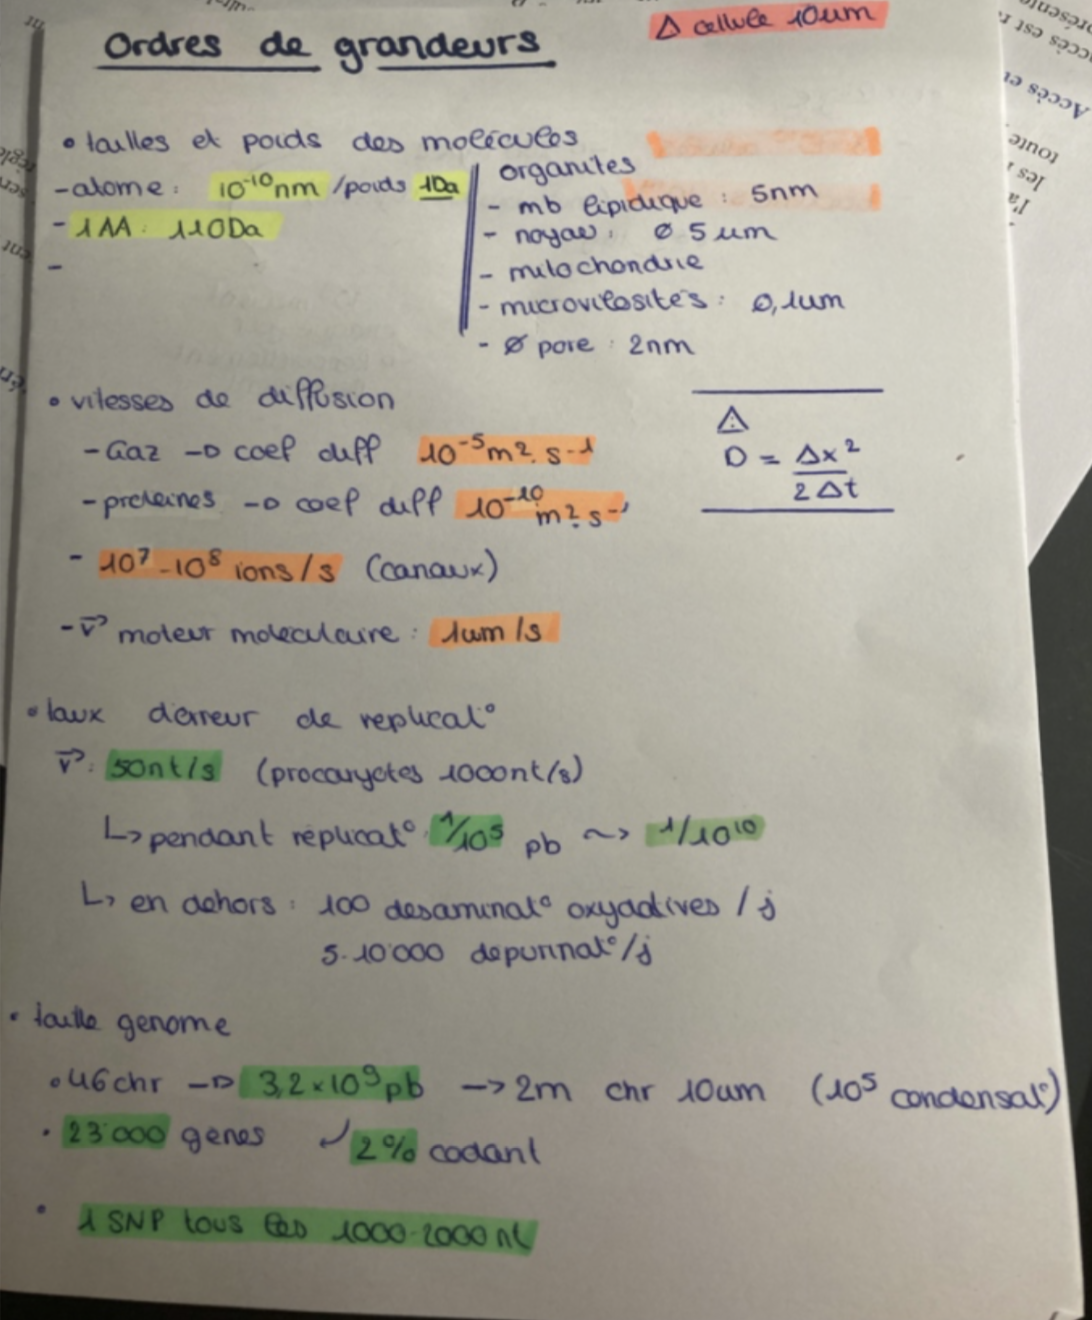
\includegraphics[width=7cm]{fiche.png}
\end{center}

Courage à vous, ce n’est pas une
période facile mais vous êtes des
guerriers !!!!!!\\


\lettrine{{\color{violet} \oldpilcrowfive}}{}
Dernier entretien de la série. L'examinateur est vraiment incroyable, et on a plus l'impression de discuter pendant 40 min que de passer un vrai oral de bio basé sur nos conséquences. \\
J'ai pioché 3 sujets complétement étranges et qui ne me mettaient pas du tout en confiance (Orage cytokinique et cancer ? SIDA ?). Il m'a très gentiment laissé repiocher jusqu'à ce que je tombe sur un sujet bien bateau : "Gènes et évolution des génomes". Je lui ai sorti un plan très peu structuré, avec des schémas de chromosomes, où je racontais globablement ce qui me passait par la tête :

\begin{enumerate}
\item Microinstabilité satellite
\item Remaniements chromosomiques
\item Évolution et pression de sélection (où j'expliquais la méiose et la fécondation ?)
\end{enumerate}

\vspace{.25cm}

Après avoir écrit ce ravissant plan au tableau, j'ai présenté mon sujet pendant une dizaine de minutes. Lui et moi voyions bien que ce n'était absolument pas préparé, mais il m'a laissé finir. Nous avons donc très vite enchaîné sur des questions de réflexion, qui ressemblaient plus à une discussion qu'autre chose, je n'ai pas vu le temps passer et c'était vraiment très agréable. Après m'avoir demandé rapidement qui j'étais et ce qui m'intéressait dans la vie (questions que je n'ai pas eues dans mon entretien de motivation), il a axé ses questions sur de la génétique des populations et de l'évolution. On avait l'impression qu'il réfléchissait en même temps que moi, que lui non plus n'avait pas la réponse et que tout ce qui importait était la réflexion. \\

Il m'a demandé quelques ordres de grandeur sur le génome, sur les temps caractéristiques en évolution... Je n'y connais absolument rien en génétique, mais je crois que c'est ce qu'il cherchait. Il m'a demandé aussi ce qui se passerait si on scindait une population en 2 (dérive génétique ?) et ce sur quelle échelle de temps. Il voulait aussi savoir ce que je pensais de la maladie, notamment en virologie, et s'il était envisageable qu'on soit un jour vacciné contre tout : les maladies disparaitraient-elles ? Certaines questions étaient parfois plus axées philo que bio, c'était assez étonnant : l'homme doit-il maîtriser la nature ?..\\

Je suis sorti assez content de cet oral, je n'avais pas beaucoup de connaissances mais nous avons tout de même pu avoir une vraie discussion, nous poser des questions sérieuses et pertinentes. L'interrogatoire était vraiment super bien mené. Niveau préparation, je pense qu'il est toujours pertinent d'avoir revu tout le programme bio de BCPST/P1, mais avec cet examinateur, la culture générale et la réflexion comptent aussi énormément, pouvant expliquer les sujets un peu hors-programme au premier abord. \\

\lettrine{{\color{yellow!80!black} \oldpilcrowfive}}{}
J’ai eu un sujet sur \textbf{la variabilité de la synthèse protéique et la régulation de la transcription} (pas exactement ça mais dans le style, c’était assez classique). L’oral de bio est celui que j’ai le plus aimé, l’idée c’est vraiment de vous éclater en discutant de sujets qui vous passionnent autour de la bio. La partie khôlle de prépa n’est là que pour construire l’entretien dessus, car l’examinateur assume qu’en médecine on a déjà plein de connaissances acquises par cœur, l’objectif étant à présent de voir ce qu’on sait en faire. Le meilleur conseil que je peux vous donner en bio, en dehors de faire une présentation potable et de réfléchir à voix haute aux questions qu’on vous aura données auxquelles vous n’aurez certainement pas la réponse, c’est de vous-même orienter l’entretien vers votre domaine de prédilection et de PROFITER. L’examinateur est lui-même ici parce qu’il adore discuter avec des étudiants passionnés, et de montrer cet intérêt et de mener la conversation vers ce qui vous plaît vraiment vous évitera les questions bidon du type : combien il y a-t-il de mitochondries dans un fibroblaste ? Perso j’ai pu avoir une discussion très intéressante sur les CAR-T et le cancer. Note : 16.\\

\newpage
\lettrine{{\color{violet} \oldpilcrowfive}}{}
\textbf{Sujets tirés :} \uline{La communication intracellulaire} ou \uline{les antibiotiques}\\
\textbf{Sujet retenu : communication intracellulaire}\\

Voici mon plan :

\begin{enumerate}[label=\textcolor{red}{\bf \Roman*.}]
    \item {\bf\color{red} La communication intracellulaire permet le transport et bonne localisation des constituants cellulaires}
    \begin{enumerate}[label=\alph*)]
        \item Communication impliquée dans le bon adressage des protéines aux compartiments cellulaires
        \item Le transport intracellulaire permet la communication entre les composants cellulaires
    \end{enumerate}
    \item {\bf\color{red}L’émission de signaux en réponse aux dommages à l’ADN, un élément central de la communication intracellulaire}
    \begin{enumerate}[label=\alph*)]
        \item Les différents types de dommages à l’ADN
        \item La cascade de signalisation des dommages de l’ADN
    \end{enumerate}
    \item {\bf\color{red}Les conséquences cellulaires de la voie de signalisation des dommage à l’ADN}
    \begin{enumerate}[label=\alph*)]
        \item Arret du cycle cellulaire
        \item Déclenchement de l’apoptose
    \end{enumerate}
\end{enumerate}

Quant à la partie questions, le prof a commencé par des questions assez simples faisant appel à des connaissances notamment sur les récepteurs à tyrosine kinase et leurs modes de transduction, aux autres types de récepteurs et a ensuite élargi le sujet en posant des questions sur d’éventuelles implications physiopathologiques/pharmaceutiques et d’imaginer des approches pour l’étude ou le développement de médicaments concernant des altérations de différentes voies de signalisation.\\
L’examinateur est très aimable et met à l’aise mais il sait aussi rester neutre donc il est difficile de savoir si ce qu’on dit est pertinent ou si on est complètement à côté de la plaque.\\



\lettrine{{\color{yellow!80!black} \oldpilcrowfive}}{}
\uline{Sujets :} Auto-immunité / immunité adaptative / \textbf{Inflammation (retenu)}\\
Alors, oui j’ai pioché tous les sujets d’immuno du paquet... alors que j’avais révisé... tous sauf l’immuno. Il m’a donc laissé pioché 3 sujets (quand il a vu ma tête), mais j’ai réussi à piocher le troisième sujet d’immuno. Si si, Je pleurais un peu intérieurement.\\
Il m’a rassurée en m’expliquant que la présentation c’est juste pour introduire la discussion, le sujet et que c’était vraiment la discussion qui vient après le plus important. Retenez bien ça !\\
J’ai jeté au brouillon tous mes souvenirs de l’inflammation depuis la terminale à la P2 et ensuite j’ai organisé un plan autour de ça. J’étais assez vague parfois (à mon avis) et dès que il y avait quelque chose que je connaissais bien, je fais une sorte de « zoom » dessus, pour étaler mes connaissances etc... Donc je crois que j’ai tenu 15min.\\
Le prof commence par se présenter et vous demande de vous présenter, on a même parlé de ce que je faisais pendant mon stage. Ça met vraiment à l’aise. Il me répète que la présentation n’est pas le plus important etc...\\

\uline{\textbf{Petite intro :}} \\
$\longrightarrow$ Définition de l’inflammation : réaction stéréotypée (rougeur / chaleur / douleur / oedème) mise en place par l’organisme face à une agression extérieur (infection) ou intérieure (cancer)\\

\uline{\textbf{Problématique :}} Quels sont les mécanismes de la réaction inflammatoire ?\\
C’est un peu bateau, j’avais pas trop d’inspiration et je m’étais plutôt concentrée sur le contenu, en me disant que je verrai après pour la problématique. Ne perdez pas du temps dessus, si ça vous n’avez rien en tête. Préparez d’abord votre plan et voyez ce qui ensuite peut bien marcher.\\

\begin{enumerate}[label=\textcolor{red}{\bf\Roman*.}]
    \item {\bf\color{red}Les acteurs de la réaction inflammatoire}
    \begin{enumerate}[label=\alph*)]
        \item Signaux de danger : PAMP / DAMP (Gram + gram - etc) reconnus par PRR / TLR / NLR
        \item Acteurs cellulaires : PNN / PNE / PNB / CPA / Macrophages (J’ai rapidement passé en revue le rôle de chacun)
        \item Inflammasome : NF$\kappa$B / IL1 / caspases\\
        {\color{green!60!black}$\longrightarrow$ \textit{(j’ai détaillé le système caspasaine / calpastatine parce que je l’avais vu dans mes révisions, donc autant que ça serve à quelque chose)}}
        \item Acteur soluble, le complément : 3 voies (classique / alterne / lectines) C6/7/8/8 = Complexe de lyse membranaire et C3a et C5a très inflammatoires.\\
        {\color{green!60!black}\textit{$\longrightarrow$ Je n’ai pas présenté toute le cascade, et ce n’est certainement pas ce qu’ils attendent de nous ! Ne vous embourbez pas dans des détails superflus. J’avais un schéma franchement pas beau sur le brouillon d’un épithélium avec une épine, 3 cellules qui se baladent, un vaisseau et une bactérie avec des triangles sur la membrane (vous voyez le genre). Essayez d’avoir quelque chose d’assez claire, car il nous demandait de lui montrer nos schémas sur le brouillon et pas de les refaire au tableau.}}
    \end{enumerate}
    \item {\bf\color{red}Recrutement des cellules immunitaires sur le lieu de l’inflammation}\\
    {\color{green!60!black}\textit{$\longrightarrow$ J’ai détaillé les cytokines / chémokines, et j’avais fait le schéma sur le brouillon roulement / reptation et touticouanti des leucocytes.}}
    \item {\bf\color{red}Rôle de l’inflammation dans les pathologies}\\
    {\color{green!60!black}\textit{$\longrightarrow$ C’était plus une ouverture qu’une vraie 3ème partie. J’ai pris pour exemple différentes pathologies vues en cours, qui avaient un lien avec l’inflammation.
    \begin{itemize}
    \item Inflammation et cancer $\Rightarrow$ L'’inflammation est-elle favorable ou défavorable ? 
    \item MICI : Maladie Inflammatoire Chronique de l’Intestin $\Rightarrow$  Interaction entre microbiote et système immunitaire 
    \item La goutte : Rôle de l’inflammasome, et traitement : Inhibiteur d’IL1-RA
    \end{itemize}}}
\end{enumerate}

Il m’a dit : « Bon bah c’était plutôt pas mal pour quelqu’un qui n’avait pas préparé ! » et on est passé aux questions :\\

\begin{enumerate}[label=\blacksquare]
    \item \uline{\textbf{De cours :}} 
    \begin{itemize}
        \item "Pourquoi les cytokines ont-elles une durée de vie aussi faible ?" \\
        $\longrightarrow$ soit $\approx$ 30min, je l’avais dit dans l’exposé, rappelez-vous, ils kiffent les ordres de grandeur, donc plus vous en dites dans l’exposé, moins ils vous en poseront — je pense — dans la période des questions
        \item "Une fois dans le vaisseau sanguin, les chémokines, avec le flux sanguin, risquent d’être emportées, donc quand elles vont se fixer sur les leucocytes, ne risquent-elles pas d’être « décalées » par rapport au site de l’inflammation ?"\\
        $\longrightarrow$ J’ai expliqué que d’une part le flux était presque nul près de la paroi au niveau de l’endothélium et d’autre part, le roulement des leucocytes se fait à l’état basal, cad sans inflammation, en état de surveillance, lorsque les chémokines passent l’endothélium, elles rentrent rapidement en contact avec un leucocyte, donc avant de se retrouver au milieu du vaisseau où le flux est important.\\
        J’ai dit que comme c’était des molécules solubles, elles étaient instables en milieu aqueux. (Je sais pas si c’est la réponse)
    \end{itemize}
    \item \uline{\textbf{Le reste :}}  Je vais essayer de retranscrire le reste sous forme de questions-réponses, mais c’était vraiment plus un échange :
    \begin{itemize}
        \item "Vous avez dit que vous aimiez la rhumatologie, pourquoi est-il important de savoir reconnaitre les signes de la réaction inflammatoire dans cette discipline ?"\\
        $\longrightarrow$ J’ai dit que cela permettait d’identifier différentes pathologies mécaniques VS inflammatoires, donc différentes origines etc... Et que l’inflammation pouvait aussi aggraver une pathologie comme l'arthrose.\\
        \item "Vous avez parlé d’inhibiteur d’IL1 dans le traitement de la goutte, ce traitement permet-il de guérir la pathologie ou l’inflammation ?\\
        $\longrightarrow$ Cela permet juste de diminuer les effets de l’inflammation, notamment la douleur, mais pas l’origine de la pathologie étant l’excès d’acide urique.
        \item "Si ça ne permet pas de guérir la pathologie, alors pourquoi ce traitement est-il utilisé ?" \\
        $\longrightarrow$ J’ai dit que la goutte pouvait très bien être occasionnelle (quelqu'un qui a mangé trop de viande) donc traiter les symptômes inflammatoires est une bonne solution dans ce cas-là mais qui ne s’appliquerait pas à un patient qui fait des crises de gouttes à répétition.\\
        J’ai souligné l’importance d’identifier la source d’une pathologie et de traiter cette dernière et pas seulement l’inflammation.
        \item On en est venu à relever la controverse des anti-inflammatoires, qui venaient masquer une pathologie en éteignant les symptômes inflammatoires, alors que l’inflammation est une réaction « physiologique » de l’organisme mise en place pour nous alerter d’un problème. J’ai cité l’exemple de l’entorse : si on prend des AINS, on ne la sentira plus, mais les ligaments continuent de se détruire, et ça deviendra irréversible etc...\\
        Cependant, l’inflammation peut devenir pathologique, d’où l’intérêt des AINS, qui est le seul traitement antalgique ciblant l’inflammation par l’inhibition des prostaglandines. \\
        Au final, ça m’ait venue après mais j’aurais pu dire : « Les antibiotiques c’est pas automatique, et les anti-inflammatoires, c’est pas obligatoire ». C’est plus ou moins ce que j’ai dit pendant l’oral, mais en moins stylé.
        \item Il a abordé la polyarthrite rhumatoïde (PR) comme exemple. Donc on a un peu parlé de maladie auto-immunes, et de mécanismes. J’ai dit que il y avait des mécanismes directs comme avec la PR mais aussi parfois indirects comme avec le lupus.
        \item Comme j’ai dit que je voulais faire de la médecine aérospatiale, il m’a demandé le rôle de l’inflammation en apesanteur. Il m’a un peu guidée pour me faire dire qu’en apesanteur, comme on n’a plus de contraintes, qui permettent justement de modeler le cartilage, celui-ci risque de « grandir » et donc être source d’inflammation au retour sur terre par exemple.
        \item "Vous avez parlé des MICI, que savez-vous ? D’où connaissez-vous cette pathologie ?"\\
        $\longrightarrow$ J’ai expliqué que ces pathologies avaient des causes environnementales, auto-immunes, et de déséquilibre avec le microbiote. J’ai dit que j’avais découvert cette pathologie sur internet parce que ça m’intéressait et lors de mon stage en soins infirmiers au service de chirurgie colorectale.
        \item Du coup on a fait une grosse parenthèse stage de médecine et m’a demandé quelles pathologies il y avait dans le service : Maladie de Chron, RCH et cancer colorectaux.
        \item "Stades de polype ?"\\
        $\longrightarrow$ J’ai dit que pour le coup c’était plus le stade carcinose péritonéale (donc très avancé) et j’ai fini par décrire l’opération à laquelle j’avais assisté une CHIP (Chimiothérapie Hyperthermique Intra-Péritonéale). Rien à voir avec l’oral, très clairement, mais il était super intéressé.
        \item Puis on est revenu au sujet : "Vous parlez d’interaction avec le microbiote, pourquoi ?"\\
        $\longrightarrow$ J’ai parlé des greffes de matières fécales qui prouvaient qu’il y avait bien une interaction entre le système immunitaire et le microbiote, et une notion d’équilibre / déséquilibre. Et on a parlé de ça pendant plusieurs minutes. J’ai abordé les complications puisqu’en effet si cellule de soi (CMH) alors peut-être microbiote du soi, donc rejet de greffe etc... Il m’a dit que, oui, ça existait et qu’il pouvait y avoir des rejets.
        \item Il m’a demandé si j’avais vu ça en cours. J’ai dit que je ne m’en rappelait pas, sûrement un reportage mais si ça se trouve, c’était peut-être un Sciences et Vie Junior. Mais pas en cours étant donné que l'UE de digestif est en D1 dans ma fac. Il était un peu déçu aha, parce que si c’était dans nos cours, ça aurait voulu dire que la recherche dans ce domaine là avait beaucoup avancé. En tous cas, d’après lui beaucoup de recherche sont faite dans le domaine.
    \end{itemize}
\end{enumerate}


« Franchement, pour quelqu’un qui n’avait pas préparé l’immunologie, c’est tout à votre mérite ! » (Bon j’ai su que ça avait peut-être mal commencé mais très bien terminé, donc faut surtout pas vous décourager et aller au bout, de belles surprises vous y attendent peut-être !).\\

Je lui répète que j’étais un peu frustrée parce qu’il y avait d’autres sujets où je possédais des connaissances très précises alors que là j’étais parfois un peu vague comme il l’avait sûrement constaté. J’ajoute en rigolant que si j’avais vraiment révisé l’immunologie comme le reste, je lui aurait dessiner toute la cascade enzymatique du complément. Ça l’a fait rire aussi.\\
Il m’accompagne dehors et dernière question sur mon stage de recherche (dans le couloir mdr), il voulait savoir si il y avait des femmes dans notre étude parce que leur adaptation était différente etc... Bref, ayez confiance en vous, même si vous avez l’impression de ne pas avoir révisé quelque chose, vous savez plein de choses, il n’y a plus qu’à leur montrer !\\


\lettrine{{\color{violet} \oldpilcrowfive}}{}
L’examinateur commence par nous expliquer le déroulé de l’épreuve et sait vraiment nous mettre à l’aise, ce qui fait que nous avions plus ou moins tous un bon ressenti en sortant. Je m’étais préparée à cette épreuve en rédigeant un plan de chacun des sujets qui tombaient le plus fréquemment. Je me suis basée sur le livre de BCPST et mes cours de PASS.\\


Sujets : \textbf{La phagocytose} ou $\underbrace{\textbf{La relation structure-fonction des protéines}}_{\text{choisi}}$

J’avais préparé le second sujet, que j’ai donc choisi sans trop hésiter.\\

\uline{\textbf{Problématique :}} Comment les protéines adoptent-elles des conformations uniques et exercent-elles des fonctions multiples nécessaires à la survie d’un organisme ?\\

\begin{tikzpicture}
\draw (0,0) node{
\begin{minipage}{0.7\linewidth}
\vspace{0cm}
\begin{enumerate}[label= \textcolor{red}{\bf \Roman*.}]
    \item \textcolor{red}{\bf De la structure primaire à la structure quaternaire des protéines}
    \begin{enumerate}[label=\alph*)]
        \item Structure $\text{\romanbar{I}}^{\text{aire}}$
        \item Structure $\text{\romanbar{II}}^{\text{aire}}$
        \item Structure $\text{\romanbar{III}}^{\text{aire}}$
        \item Structure $\text{\romanbar{IV}}^{\text{aire}}$
    \end{enumerate}
    
    \item \textcolor{red}{\bf Le repliement des protéines leur permet d’acquérir une fonction spécifique}
    \begin{enumerate}[label=\alph*)]
        \item Le repliement de la protéine est encodé dans sa structure primaire
        \item Les modèles de repliement des protéines
        \item Les protéines d’aide au repliement (chaperonnes) 
        \item Dégradation par le protéasome en cas de mauvais repliement
    \end{enumerate}
    
    \item \textcolor{red}{\bf Les protéines exercent des fonctions multiples et variées au sein de l’organisme}
    \begin{enumerate}[label=\alph*)]
        \item Les protéines fibreuses structurent la cellule
        \item Les protéines globulaires jouent un rôle important dans le métabolisme
    \end{enumerate}
\end{enumerate}
\end{minipage}
};

% partie I
%% item A
\draw[->,>=latex, color=green!60!black, shift={(-1,3.6)}] (0,0) to[out=30, in=180, looseness=1] (2,.35) node[right, fill=green!5!white]{
\scriptsize
Acide aminé (structure, pttés, fonctions) + liaison peptidique
};
%% item B
\draw[->,>=latex, color=green!60!black, shift={(-0.95,3.1)}] (0,0) to[out=30, in=180, looseness=1] (2,.45) node[right, align=left, yshift=-.15cm, fill=red!5!white]{
\scriptsize 
Hélice $\alpha$, feuillet $\beta$, coudes, boucles \\[-.1cm]\scriptsize+ Association de structures secondaires en domaines
};
%%item C
\draw[->,>=latex, color=green!60!black, shift={(-0.85,2.4)}] (0,0) to[out=15, in=180, looseness=1] (2,.4) node[right, align=left, yshift=-.15cm, fill=blue!5!white]{
\scriptsize 
Maintien de la structure tertiaire par des liaisons covalentes, \\[-.1cm] \scriptsize hydrogène, ioniques (importantes pour la fonction des protéines)
};
%%item D
\draw[->,>=latex, color=green!60!black, shift={(-0.85,1.9)}] (0,0) to[out=-15, in=180, looseness=1] (2,.1) node[right, align=left, yshift=-.15cm, fill=orange!5!white]{
\scriptsize 
Association de chaînes peptidiques\\[-.1cm]\scriptsize + Assure des fonctions biologique 
};

% Partie II
%% item A
\draw[->,>=latex, color=green!60!black, shift={(4,0.5)}] (0,0) to[out=40, in=150, looseness=1] (1.8,.2) node[right, fill=green!5!white, yshift=-.5cm]{
\begin{minipage}{0.3\linewidth}
\scriptsize
Ex : hémoglobine avec importance de la séquence d’AA montrée par la seule mutation en cause dans la drépanocytose.\\
Résidus qui peuvent acquérir des modifications post-traductionnelles qui déterminent la structure de la protéine
\end{minipage}
};
%%item B
\draw[->,>=latex, color=green!60!black, shift={(2.9,-.6)}] (0,0) to[out=10, in=190, looseness=1] (3,-.6) node[right, align=left, yshift=-.15cm, fill=orange!5!white]{
\begin{minipage}{0.25\linewidth}
\scriptsize 
Séquentiel et hiérarchique, effondrement hydrophobe, entropie 
\end{minipage}
};

%Partie III
%% item A
\draw[->,>=latex, color=green!60!black, shift={(3.4,-3.6)}] (0,0) to[out=10, in=170, looseness=1] (2.5,.2) node[right, fill=blue!5!white]{
\begin{minipage}{0.3\linewidth}
\scriptsize Collagène, kératine, protéines musculaires
\end{minipage}
};
%% item B
\draw[->,>=latex, color=green!60!black, shift={(3.4,-4.4)}] (0,0) to[out=-60, in=-160, looseness=1] (2,-.5) node[right, fill=yellow!5!white]{
\begin{minipage}{0.3\linewidth}
\scriptsize
Albumine, globuline\\
Défense de l’organisme : anticorps
\end{minipage}
};
\end{tikzpicture}

\bigskip


Vinrent ensuite les questions, divisées en trois groupes :
\begin{itemize}
    \item Celles auxquelles une réponse est attendue
    \item Celles auxquelles une réponse n’est pas forcément attendue, mais plutôt un cheminement ou une/des  hypothèses
    \item Celles auxquelles personne n’a de réponse pour l’instant (conseil pour pouvoir espérer répondre correctement à une des questions \href{https://www.youtube.com/watch?v=4xmCe_PQybE}{<ici>})
\end{itemize}

\vspace{.5cm}


Voici une partie des questions que l’examinateur m’a posées :
\begin{itemize}
    \item Comment déterminer la structure d’une protéine ?
    \item Pouvez-vous citer quelques modifications post-traductionnelles ?
    \item Comment expliquer la diversification du rôle des protéines depuis la cellule procaryote à la cellule eucaryote ? 
    \item Quelle conception avez vous d’une protéine ? (\href{https://drive.google.com/file/d/1yT1XqiO7yJkoMji1EzFvYaB0gDA03Eax/view?usp=sharing}{Je vous laisse philosopher à votre guise})
\end{itemize}



\newpage

\subsection{Physique (coefficient 1)}

\subsubsection{Déroulement de l'épreuve}

L’épreuve de physique est moins guidée que celle de biologie, le professeur te laisse quelques minutes pour réfléchir de ton côté sur un sujet plus ou moins ouvert (en général il y a une à quelques questions pour guider la réflexion), puis tu passes au tableau et commences la résolution. Mais la majeure partie de l’épreuve est surtout une discussion avec l’examinateur qui te pose des questions pour t'orienter à partir du moment où tu bloques.\\

La petite particularité de cette épreuve est que l’examinateur (notre année en tout cas) ne respecte pas tellement les 30 minutes théoriques que dure l’épreuve, ce qui entraîne beaucoup de retard pour les candidats suivants.\\

Théoriquement, le programme comprend l’enseignement de spécialité de terminale en physique-chimie, mais nous te conseillons de maîtriser aussi les notions de première année de médecine et quelques notions de prépa PCSI, le programme de médecine étant différent selon les facultés. Voici une liste des quelques domaines clés à maîtriser qui retombent souvent aux oraux :

\begin{itemize}
\item Optique ondulatoire et optique géométrique de lycée et de PASS, à compléter avec des exercices de prépa
\item Mécanique du point (bilans de forces, travail, vitesse, accélération, $2^e$ loi de Newton...) : programme de lycée et de PASS complété avec des exercices de première année de BCPST ou PCSI (en particulier la résolution des équations différentielles)
\item Mécanique des fluides (principe fondamental de l’hydrostatique, loi des gaz parfaits, loi de Poiseuille, effet Venturi, lois de Hooke et de Laplace, transport membranaire et équilibre de Starling, poussée d’Archimède)
\item Frottements
\item Mécanique des ondes : ondes électromagnétiques et mécaniques, ondes sonores, effet Doppler
\end{itemize}

Il est aussi important de maîtriser les différents outils mathématiques de résolution de problèmes physiques : trigonométrie, géométrie euclidienne de lycée, résolution d’équations différentielles, dérivation...\\

Nous te conseillons aussi de bien t'entraîner sur des exercices de khôlles de prépa puisque l’oral est vraiment du même format. Si tu arrives à te trouver un examinateur qui te fasse passer un oral blanc avec un tableau (un ami en prépa par exemple) c’est l’idéal, puisque tu n’as normalement pas du tout l’habitude de ce format d’épreuve et devoir dérouler son raisonnement sur un tableau pour la première fois le jour J peut parfois être déroutant.

\subsubsection{Témoignages}

\lettrine{{\color{violet} \oldpilcrowfive}}{}
Premier oral de la série. Malgré des horaires assez honnêtes, j'ai encore l'impression de ne pas être totalement sorti de mon lit. Après 5 cafés et 3 passages d'eau glacée sur la tête, je transpire toujours autant mais ne sais toujours pas comment je m'appelle. L'examinateur, très sympa et probablement aussi réveillé que moi m'appelle et il faut y aller : \\

\textbf{Modélisation et analyse d'une pseudo-molécule/noyau et ses électrons}. On étudie 3 masses $m_1, m_2, m_3$ maintenues entre elles par deux ressorts $k$ (entre $m_1$ et $m_2$) et $k'$ $(m_2 \rightarrow m_3)$. En gros l'examinateur laisse une dizaine de minutes pour se préparer sur brouillon, il y a pas mal de questions sur la feuille, mais l'objectif est principalement d'appréhender le système, les forces en présence, les ordres de grandeur... J'arrive lamentablement à écrire les équations nécessaires pour les questions 1 et 2 (avec une petite erreur de signe en bonus), puis l'examinateur propose d'étudier l'exercice tous les 2 en reprenant depuis 0, et je lui présente rapidement mes résultats.\\

L'objectif est d'étudier le déplacement de l'ensemble du système suite à une petite perturbation (par exemple sur $m_1$). On commence doucement avec les définitions d'un ressort, le bilan des forces en présence, les "contraintes" qu'on peut supposer (ici les masses ne peuvent pas se croiser, on aura toujours l'ordre $m_1, m_2, m_3$)... Contrairement aux notations que j'avais proposées, on pose $x$ la distance entre $m_1$ et $m_2$, et $x'$ la distance $m_2$ et $m_3$ : tout ce que j'avais préparé va devoir être "repensé". Comme l'examinateur voit que je suis un peu perdu, que j'ai du mal à me poser et aligner 2 mots, il passe en mode accompagnateur et me guide tout le long de l'exercice.\\

\begin{center}
\begin{tikzpicture}
\draw[fill=black](0,0)circle(.25)node[below=.3cm]{$m_1$};
\draw[spring] (0,0) --++ (2,0);
\draw[fill=black](2,0)circle(.25)node[below=.3cm]{$m_2$};
\draw[spring] (2,0) --++ (2,0);
\draw[fill=black](4,0)circle(.25)node[below=.3cm]{$m_3$};

\draw[|-|](0,.5)--++(2,0)node[midway, above]{$x$};
\draw[|-|](2,-.85)--++(2,0)node[midway, below]{$x'$};
\end{tikzpicture}
\end{center}

En réfléchissant tous les deux et en se plaçant dans un système avec que des forces conservatives, on étudie tous les mouvements d'un point de vue Newtonien (conservation de la quantité de mouvement, en découlent des infos sur l'accélération du système, et on réintègre tout ça pour retrouver les positions) et on arrive à un système sur 5 inconnues ($m_1$, $m_2$, $m_3$, $x$, $x'$) avec 5 équations, qu'il faudrait résoudre pour pouvoir enfin répondre aux questions de l'exercice. Comme l'examinateur voit bien que je n'arriverai pas à le résoudre formellement, il commence à tout faire à ma place, m'expliquant qu'il y a beaucoup trop de calculatoire dans ses questions. \\

Au bout d'un moment, je comprends qu'il veut m'amener vers un système oscillatoire depuis le début, et qu'il faut absolument remanier la forme des équations sur le mouvement. Je n'ai plus du tout les formules en tête, mais on arrive à quelque chose qui ressemble à une fréquence fondamentale $\omega_0$ avec des sinus et des cosinus un peu partout, et je vois qu'il a l'air tout content. Il me propose alors de passer à une autre question (alors qu'on a toujours pas résolu la première), en posant l'hypothèse que $x=\omega_0 \sin(\omega t)$, et pareil pour $x'$ comme l'un et l'autre sont couplés. En réinjectant ceci dans notre système initial, et en manipulant les équations à la louche, on arrive à montrer que la pulsation globale du système est fonction de $\omega_0$ et $\omega_0 '$.\\

Pour le dernier quart d'heure, on essaye de prendre un peu de hauteur sur l'exercice, pour voir à quoi il pourrait servir en médecine, ou ce qu'il pourrait modéliser. Je lui dis que ça me fait penser à des liaisons moléculaires, et qu'on se sert probablement des pulsations propres à chaque liaison en RMN. S'ensuit une discussion (je l'écoutais surtout) sur plein de choses absolument géniales - je cite : levée de dégénérescence, liaisons couplées...\\

Comme exemple de questions qu'il m'a posées à la fin : pourquoi les liaisons vibrent-elles ? J'ai essayé de le prendre d'un point de vue atomique, en lui servant un truc sur les OA liantes et anti-liantes; il attendait juste le mot "puits de potentiel", que la liaison a un point d'équilibre stable sur une longueur spécifique, et qu'elle vibre simplement autour.\\

Je sors de là en n'étant pas forcément mécontent pour un premier oral, même si j'ai l'impression d'avoir surtout regardé l'examinateur résoudre mon problème. N'ayant fait que la moitié des questions, je savais que l'optique de l'oral n'était pas de tout résoudre, mais de voir juste comment je peux réfléchir. \\

Si vous voulez trouver des exos similaires, on peut en trouver plein sur les oscillateurs couplés. Niveau préparation, de la physique de lycée bien poussée ou première année de prépa devrait vous préparer à la plupart des problèmes rencontrés. Surtout l'examinateur s'adapte extrêmement vite et saura poser les bonnes questions, il est vraiment génial.\\


\lettrine{{\color{yellow!80!black} \oldpilcrowfive}}{}
C’était un exercice sur la tension de surface entre autre. Il y avait un énoncé avec environ 15min pour
lire et réfléchir et des questions après. C’est pas forcément la peine de réfléchir à toutes les
questions parce qu’il n’y aura pas forcément le temps d’aller au bout et le temps de préparation c’est
du temps perdu pour l’oral. Ça s’est plutôt bien passé. L’examinateur était très sympa, il laissait
expliquer ce qu’on voulait en nous aidant ni trop tôt ni en nous laissant trop galérer. J’ai fait un
schéma, puis une mise en équation, il m’a aussi posé quelques questions en dehors de celles
préparées, c’était un peu une discussion. C’est utile de bien écouter ce qu’il dit car c’est souvent ce
qui est important pour la suite de l’exercice.\\

\lettrine{{\color{violet} \oldpilcrowfive}}{}
Mon sujet portait sur le cratère d’une météorite qui se trouve en Arizona (USA).
Il s’est formé à la suite de l’impact d’une météorite de 50 m de diamètre et de 300 000 tonnes arrivant avec une vitesse de 20km/s. Il a laissé ce cratère derrière lui de 1,2 km de diamètre. L’objectif était de retrouver sa profondeur.\\

Cherchez un peu ;)

\begin{center}
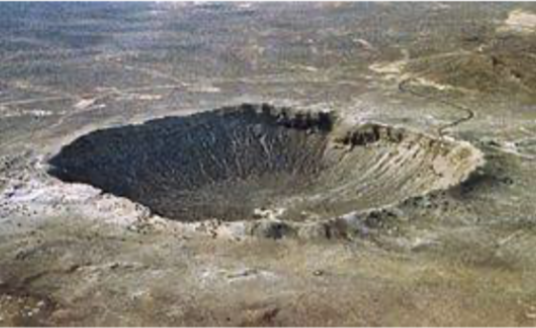
\includegraphics[width=5cm]{cratere.png}
\end{center}

Alors je ne pense pas que c’était l’exercice le plus dur mais j’ai mis du temps avant d’arriver à la solution. L’examinateur était trop sympa, j’ai passé un très bon moment alors que c’est l’épreuve que je redoutais presque le plus (je suis passée l’avant dernière et tous les gens avant moi n’arrêtaient pas de dire que c’était horrible et tout).\\

\textbf{Commencez par faire un schéma !!!!! C’est obligatoire !} Après commencez à parler, expliquez le contexte, les paramètres qu’il faut prendre en compte, les idées que vous avez, etc.\\
Mon idée de base était de partir sur les forces. Donc j’ai parlé des paramètres de la météorite : comment elle entre dans l’atmosphère, sa perte de masse, sa vitesse… et là on a commencé à discuter de comment les astronautes font pour revenir sur terre, des matériaux qui résistaient à l’entrée dans l’atmosphère et tout. Puis j’ai parlé des paramètres du sol.\\

En fait, je pensais rechercher la force d’impact pour avoir la pression qu’avait exercé la météorite sur le sol pour retrouver la profondeur.\\
On a enchainé avec une discussion au tout de la théorie de la force de pression. Il me posait des questions et me donnait des pistes. Je pense qu’il a énormément testé ma capacité de raisonnement.\\

Bref au bout d’un moment il m’a fait dire (littéralement) qu’il fallait que j’utilise les énergies (je me
suis sentie trop bête).


$$
\begin{cases}
E_c= \frac12mv^2\\
E_{pot,g} = mgh
\end{cases}
$$


On a approximé qu’il n’y avait pas de perte d’énergie, donc :

$$
\begin{aligned}
    E_c=E_p
    \iff &\frac12mv^2=mgh\\
    \iff &h=\frac{v^2}{2g}
\end{aligned}
$$

On trouve ainsi la hauteur (et donc la profondeur) !\\

Ensuite on a parlé de la dissipation de l’énergie lors de l’impact :
\begin{itemize}
    \item Frottement
    \item Thermique
    \item Tremblements de terre
    \item ...
\end{itemize}

Comme vous avez pu le comprendre, je n’ai pas effectué cet exercice toute seule mais je n’ai jamais abandonné, j’ai gardé le sourire et l’envie d’y arriver tout le long et je n’ai pas hésitez à dire ce que je pensais tout haut et à poser des questions. C’est votre curiosité et votre entrain qui feront la différence.\\

Courage à vous, ce n’est pas une période facile mais vous êtes des guerriers !!!!!!

\newpage

\lettrine{{\color{yellow!80!black} \oldpilcrowfive}}{}
J’ai commencé l’entretien par dire à l’examinateur que, venant de la faculté de \href{https://www.youtube.com/watch?v=LkUfrAJbLus}{Marseille}, les mathématiques avaient cessé d’exister pour moi au lycée (coucou les Marseillais :) ).\\
En effet, nous ne savions même pas ce qu’était une équa diff alors que dans d’autres facultés tout le monde sait te faire des calculs dont tu ignores l’existance même. Partant de là, on a abordé l’exercice « sans calculs ». En effet, j’avais parfaitement compris l’exercice, je savais comment le résoudre, et intuitais les résultats que j’étais censé trouver, seulement je n’avais pas les outils mathématiques pour le faire. \\
L’entretien s’est très bien déroulé à partir de là car l’examinateur avait compris que j’avais moi-même compris, donc on est parti sur des questions qui n’avaient rien avoir du type : « qu’est-ce que la lumière ? ». En somme, le fait de ne pas avoir les outils mathématiques n’est pas rédhibitoire, mais tout de même assez pénalisant étant donné que l’objectif est en partie de vous voir faire des calculs. Du coup si vous venez d’une fac où vous avez très peu ou pas de maths, mettez-y-vous dès que possible (vous partez avec une longueur de retard par rapport aux autres donc faites-le savoir en début d’entretien si c’est votre cas, sans abuser non plus car en lisant ceci vous êtes prévenus et pouvez vous-y préparer). Note : 14 (on ne peut pas en demander plus quand on se souvient à peine de comment \href{https://www.youtube.com/watch?v=Z3vKJJE57Uw}{faire une intégrale}).\\


\lettrine{{\color{violet} \oldpilcrowfive}}{}
L’examinateur était très sympa et mettait à l’aise.\\
Mon sujet était composé de 9 questions liées entre-elles pour comprendre comment se forment les gouttes d’eau sur une toile d’araignée. Lors de la préparation je n’ai fait que les 3 premières questions car je ne comprenais pas très bien ce qui était demandé après.\\
Lors du passage au tableau, le prof a pu reformuler les questions qui me bloquaient, ce qui m’a permis d’avancer jusqu’au bout.
Je n’ai malheureusement pas le détail des questions mais elles étaient plutôt simples et pas trop calculatoires/mathématiques, il s’agissait de rappeler des formules d’interaction électrostatique et faisaient appel aux notions de tension de surface et énergie.\\
D’une part, il fallait voir que les molécules d’eau à l’interface eau/air établissaient des liaisons hydrogènes uniquement dans une direction (vers l’eau et pas vers l’air). Ceci se traduit par une énergie correspondant à cette différence liaisons hydrogène à l’origine de la tension de surface. Ensuite, il fallait trouver la situation la plus énergétiquement favorable le long du fil en prenant en compte la « mouillabilité » du fil et son diamètre.\\
Globalement, l’exercice faisait appel à des notions de terminale scientifique et était très guidé et progressif (9 questions).\\

\lettrine{{\color{yellow!80!black} \oldpilcrowfive}}{}
Un exercice avec une histoire de flux thermique... j’avais jamais vu ça. Ce qui permettrait d’estimer la distance entre le soleil et la Terre en gros... Je n’avais rien compris. J’ai résolu les 2 premières questions, je crois, AVEC le prof, j’ai pas l’impression d’avoir fait grand chose en fait. J’ai pas vu beaucoup de physique dans l’exo, surtout de maths, avec équations partielles secondes, le genre de truc que j’ai fait pendant un mois dans ma vie, au lycée, donc il y a plus de 2 ans. Autant vous dire que j’étais paumée. Je dirais qu’il faut s’entrainer sur quelques exos pour être à l’aise. J’essayais de montrer autant que possible que je comprenais ce que le prof me disait / faisait et je refaisais la 2ème inconnue après qu’il m’ait montré avec la première. A défaut, il faut au moins être calé sur ses dérivés / primitives.\\
Il m’a posé quelques questions de culture générale en lien avec l’exercice : rayonnements UV, couche d’ozone, réchauffement climatique etc...\\
Il m’a demandé d’où je venais, car en fonction des facs, on n’a pas eu le même programme de physique, voire pas de physique en P1 en fait, ce qu’il en prenait compte. A Paris typiquement, ils ont un module de biophysique ET un module de physique. Je pense que pour vos révisions de physique, ça peut être bien de jeter un oeil au programme de physique de P1 de Paris pour se mettre à niveau si vous êtes d’une autre fac. C’est un oral qui est très long, 40-45min ! Donc faîtes gaffe à votre train / avion si vous passez en fin d’aprem, mais surtout il faut pas lâcher !\\
Et c’est bien de savoir représenter le problème sous forme de schéma, c’est plus facile pour visualiser et discuter.\\

\lettrine{{\color{violet} \oldpilcrowfive}}{}
C’était mon dernier oral, et l’examinateur qui passait plus de trente minutes avec chacun d’entre nous (50 min environ) avait accumulé pas mal de retard. De mon point de vue cela est une bonne chose, on a vraiment le temps d’exposer notre réflexion et de répondre à plusieurs questions. J’ai senti avoir pu montrer que j’avais des bases solides sur les notions que nous avions abordées. \\

Avant de me tendre le sujet, l’examinateur m’a demandé si j’avais suivi l’école de février. C’était mon cas, il a donc choisi un sujet avec des notions qu’on y avait traitées. L’exercice portait sur le phénomène de cavitation que peuvent effectuer les crevettes-pistolet, pour attaquer ses proies.  Cette crevette possède une grande pince qui peut se fermer avec une telle violence que cela crée une bulle (cette action est appelée cavitation) qui produit un son qui atteint 218 dB. Voici les questions dont je me souviens.

\begin{itemize}
    \item Peut-on dire que l’eau dans laquelle est immergée la crevette est un fluide parfait ?
\end{itemize} 

J’ai d’abord dit que la viscosité de l’eau était faible, ce qui pouvait nous permettre de considérer l’eau comme un fluide parfait. 

\begin{itemize}
    \item L’examinateur m’a donc demandé de caractériser l’écoulement de l’eau autour de la crevette et de le dessiner.
\end{itemize}

 J’ai évoqué et calculé le nombre de Reynolds qui compare l’inertie à la viscosité pour caractériser l’écoulement autour de la crevette, laminaire dans ce cas. Il fallait connaître la masse volumique et la viscosité de l’eau (globalement il y a certaines grandeurs assez indispensables à connaitre en physique, mais sinon l’examinateur vous les donnera). 

\begin{itemize}
    \item L’énoncé disait que la crevette pouvait projeter de l’eau à 100 km/h. Il fallait ensuite exprimer une différence de pression que j’ai choisie entre le point d’éjection de la pince et le point où la vitesse s’annule.
\end{itemize} 

Pour relier la vitesse et la pression, j’ai utilisé la loi de Bernoulli qui se simplifiait à altitude constante. On trouvait une pression plus faible au point d’éjection de la pince par rapport au point où la vitesse s’annule. Il fallait donner une interprétation qualitative (ce que je vous conseille de faire automatiquement après avoir trouvé un résultat) et conclure que c’était cette dépression qui permettait l’apparition d’une phase gazeuse, la bulle de vide responsable du phénomène de cavitation. 

\begin{itemize}
    \item Tracer le diagramme des phases de l’eau (avec la pression et la température) pour rendre compte de cette interprétation qualitative
\end{itemize}

J’avais rapidement revu les diagrammes de phase en travaillant la physique de BCPST1, et avec un raisonnement qualitatif sur les changements d’états à pression égale puis à température égale (et les retours de l’examinateur), j’ai tracé ce diagramme. Je souligne cela parce que je pense que c’est une bonne chose de ne pas forcément vous lancer dans un dessin ou un calcul sans exposer vos hypothèses, pour vous rendre compte de leur cohérence ou les ajuster, ce qui montre que vous pouvez raisonner. 

\begin{itemize}
    \item Connaissez-vous d’autres exemples de cavitation ?
\end{itemize}

J’ai cité les sous-marins, qui ont des hélices tournant à une vitesse assez élevée. L’exemple était correct, et ce n’est qu’en sortant que je me suis souvenue qu’on en avait parlé en cours… 

\begin{itemize}
    \item Il y avait d’autres questions sur des forces de Wan der Waals et le diagramme énergétique qui découle de l’interaction entre deux particules, sur le phénomène de tension superficielle.
\end{itemize}

J’y avais un peu réfléchi pendant la préparation (j’avais lu tout le sujet pour avoir une approche globale, je vous conseille de le faire) mais nous n’avons pas eu le temps de les aborder. D’ailleurs je déconseillerai de préparer tous les calculs pendant la préparation mais plutôt de noter des raisonnements ou des pistes de réponse à chaque question. Puis à l’oral, ne vous pressez pas pour aborder un maximum de questions mais prenez le temps d’exposer rigoureusement vos raisonnements. \\

De façon globale j’avais l’impression que l’examinateur s’adaptait beaucoup à nous, et qu’il savait très bien nous orienter pour que l’on trouve par nous-mêmes les bonnes hypothèses et les bons résultats. Je conseillerai donc d’arriver à prendre du recul au moment de l’oral, à réfléchir avec l’examinateur, et finalement vivre cet oral comme l’expérience enrichissante d’un dialogue ouvert avec un chercheur autour d’un sujet scientifique tout à fait intéressant. \\

\lettrine{{\color{yellow!80!black} \oldpilcrowfive}}{}
Etude de la mouillabilité d'une toile d'araignée. Le texte qui suit est la remise en page de photos que tu pourras retrouver \href{https://drive.google.com/drive/folders/1Nw3P73PGFFsGEVnGJiq1UKrKFstN233L?usp=sharing}{<ici>}\footnote{https://drive.google.com/drive/folders/1Nw3P73PGFFsGEVnGJiq1UKrKFstN233L?usp=sharing}.


$$
\begin{tikzpicture}
\draw (0.1,0.1) grid (3.9,3.9);
\foreach \j in {1,...,3}
    \foreach \i in {1,...,3}
    \draw (\i,\j) node{$\bullet$};
\draw[<-,>=latex, color=red] (3,1) to[out=-60, in=250, looseness=2] (5,2) node[above, xshift=2cm]{
\begin{minipage}{.3\linewidth}
\color{black} Les gouttes de rosées se posent uniquement sur les parties larges de la toile
\end{minipage}
};
\draw[->,color=green!60!black] (0.8,1) to[out=200,in=160,looseness=1] (0,-2);
\draw[color=green!60!black] (1,1)circle(0.2);

\begin{scope}[shift={(0,-3)}]
\draw[double] (0.1,0.1) grid (1.9,1.9);
\draw[fill=white](1,1) circle(0.35);
\draw[<-,>=latex](0.7,0.7) to[looseness=1, out=230, in=0] (0,0)node[left]{bourrelet};
\draw[<-,>=latex] (1.5,0.95) to[out=-90, in=180, looseness=1] (2,0.3) node[right]{joint};
\end{scope}
\draw[color=green!60!black] (1,-2) circle(0.9);
\end{tikzpicture}
$$


\underline{\textbf{Partie A :}} Etude des interactions intermoléculaires

\hspace{-1.5cm}\begin{minipage}{.6\linewidth}
\begin{tikzpicture}
  \begin{axis}[domain  = 0.5:2.3,
               samples = 100,
               xmin    = 0.3,
               xmax    = 2.3,
               ymin    = -1.4,
               ymax    = 1,
               xtick=\empty,
               ytick=\empty,
               xlabel  = {$r$},
               ylabel  = {$u$},
               extra y ticks = {0,-1},
               xlabel near ticks,
               ylabel near ticks,
               set layers,
              ] 
    \addplot[thick,
             samples=400
            ] {0.25/x^12-1/x^6};
    \draw[dashed,thin] (axis cs: 0.3, 0 )-- (axis cs: 2.3, 0);
    \draw[loosely dashed,very thin] (axis cs: 0.3, -1 )-- (axis cs: 2.3, -1);
\end{axis}
\end{tikzpicture}
\end{minipage}
\begin{minipage}{.5\linewidth}
\begin{enumerate}[label=\alph*)]
    \item Pourquoi $u\nearrow$ quand $r\to 0$ ?
    \item Quelle est la valeur de la distance de plus basse énergie ?
    \item Que se passe-t-il quand on éloigne deux atomes ?
\end{enumerate}
\end{minipage}

\bigskip

\begin{minipage}{0.3\linewidth}
\begin{tikzpicture}
\shade[inner color=blue!20!white, outer color=white] (0,0) circle(1);
\draw(0,0) node{
\chemfig{H-[1]O-[7]H}
};
\shade[inner color=blue!20!white, outer color=white] (-1.5,-1.5) circle(1);
\draw(-1.5,-1.5) node{
\chemfig{H-[1]O-[7]H}
};
\shade[inner color=blue!20!white, outer color=white] (0.6,-1.7) circle(1);
\draw(0.6,-1.7) node[]{
\chemfig{H-[2]O-[0]H}
};

\draw[densely dashed, color=red, very thick] (-0.9,-.55)--(-1.35,-1.05);
\draw[densely dashed, color=red, very thick] (-0.6,-1.8)--(-.05,-1.3);
\draw[densely dashed, color=red, very thick] (.2,-1)--(0.5,-0.5);
\end{tikzpicture}
\end{minipage}
\begin{minipage}{.5\linewidth}
Interactions entre molécules d'eau (liaisons hydrogènes)
\end{minipage}

\hrulefill\\


\underline{\textbf{Partie B :}} On donne $W=\gamma S$ l'énergie de création d'une surface $S$ eau-air.

\begin{enumerate}[label=\alph*)]
    \item Justifier que créer une telle surface coûte de l'énergie
    \item On considère une goutte entre deux surfaces (bourrelet et joint). Montrer par un raisonnement énergétique sur un petit déplacement $dx$ qu'il existe une force sur la goutte d'eau.
\end{enumerate}

$$
\begin{tikzpicture}[scale=2]
    \draw(0,0)--++(0,2);
    \draw[pattern=north west lines] (0,1) circle(0.5);
    \draw[<->] (0,0.25)--++(.25,0) node[midway, below]{$dx$};
\end{tikzpicture}
$$

\hrulefill\\
\newpage

\underline{\textbf{Partie C :}} Pression de Laplace

$$
\begin{tikzpicture}
    \shade[inner color=blue!40!white, outer color=blue!2!white] (0,-1.5) to[out=150, in=-150, looseness=1] (0,1.5) --++(10,0) to[out=-30, in=30,looseness=1] (10,-1.5)--++(-10,0);
    
    \draw (0,-1.5) to[out=150, in=-150, looseness=1] (0,1.5) --++(10,0) to[out=-30, in=30,looseness=1] (10,-1.5)--++(-10,0);
    

    \draw[dashed, fill=white] (.5,-1) to[out=150, in=-150, looseness=1] (0.5,1) --++(9,0) to[out=-30, in=30,looseness=1] (9.5,-1)--++(-9,0);
    \draw[dashed] (9.5,1) to[out=-150, in=150, looseness=1](9.5,-1);

    \draw (10,1.5) to[out=-150, in=150, looseness=1](10,-1.5);
    
    \draw[<->,>=latex](1,-1.5)--++(0,.5) node[midway,right]{$e$};
    \draw[<->,>=latex] (3,0)--++(0,1) node[midway, right]{$r$};
    \draw[densely dashed, color=black!70!white,->, >=latex] (-2,0)--++(14,0);
    
\end{tikzpicture}
$$

On considère un cable tendu de rayon $r$, entouré d'une fine couche d'eau ($e$ très petit).\\
Montrer que la pression de la couche est telle que :

$$
\fbox{$P=\frac{\gamma_{a/r}}{r}$}
$$

\newpage

\subsection{Chimie (coefficient 1)}
\subsubsection{Déroulement de l'épreuve}

A nouveau une épreuve où le professeur vérifie surtout que tu possèdes les connaissances de base les plus importantes en chimie, et pendant laquelle il va évaluer ta capacité de réflexion. L’examinateur te fournit un sujet et te laisse quelques minutes pour lire l’énoncé et élaborer des pistes de réflexion pour répondre aux questions.\\

Les sujets de chimie sont souvent composés d’une suite de 2 à 4 questions, qui peuvent être plus ou moins ouvertes en fonction du sujet. Notre année, l’examinateur ne cherchait pas forcément à nous faire répondre aux questions posées mais nous suivait dans les voies dans lesquelles nous nous engagions.\\

L’épreuve de chimie se base officiellement sur le programme de PASS. Or comme vous le savez sûrement, celui-ci diffère très largement entre les différentes facs. Il s’agit donc plutôt du programme de prépa scientifique (BCPST, voire PCSI) de première année. \uline{Les grandes thématiques à maîtriser absolument sont les suivantes :}

\begin{itemize}
\item Atomistiques et liaisons chimiques
\item Thermodynamique
\item Stéréochimie
\item Réactions acido-basiques
\item Réactions d’oxydo-réduction
\item Chimie organique (+++) : il s’agit de connaître et de savoir réfléchir sur l’ensemble des réactions vues en PASS ainsi que parfois sur des réactions de chimie inorganique (organomagnésiens très présents en prépa)
\end{itemize}

\vspace{.5cm}

\uline{Quelques conseils pour cette épreuve :}

\begin{itemize}
\item Il faut bien s’entraîner à réfléchir sur des questions ouvertes (et non pas sur des QCMs comme en PASS) : n’hésite pas à faire beaucoup d’exercices et des oraux blancs
\item Entraîne-toi à réfléchir à l’oral (plus difficile que l’on ne le croit)
\end{itemize}

\subsubsection{Témoignages}

\lettrine{{\color{violet} \oldpilcrowfive}}{}
Je suis pas forte en chimie, c’était un exercice je pense assez classique de chimie organique. On
devait passer d’une molécule à une autre (après il y avait d’autres questions mais j’ai pas eu le
temps). Je ne savais pas répondre quand il me demandait des choses sur le nom des réactions ou des
molécules, mais le plus important je pense que c’est que même si je galérais bien au début, j’ai bien
progressé au cours de l’exercice et il a dû voir que je comprenais ce que je faisais et que j’apprenais
et j’enregistrais les mécanismes. A savoir que c’est utile de réfléchir à voix haute comme ça il pourra
vous aider si vous vous trompez par exemple, ou vous encourager à continuer. Bien connaître et
savoir réfléchir sur quoi est réactif ou stable, par exemple même si je ne connaissais pas les réactions
classiques, je savais qu’un élément était nucléophile, un autre électrophile donc je pouvais supposer
des attaques…\\

\lettrine{{\color{yellow!80!black} \oldpilcrowfive}}{}
Examinateur assez particulier, qui ne parle pas beaucoup et nous laisse vraiment le temps de réfléchir dans notre coin, quitte à raconter n'importe quoi, se contredire et repartir sur le bon chemin. La phase de préparation était vraiment courte, et j'ai vraiment eu l'impression de tout faire au tableau, à dessiner médiocrement sur un tableau beaucoup trop petit. \\

Le sujet était un sujet de chimie orga assez classique, une fusion de 2 cycles assez gros et compliqués qu'il fallait expliquer. On avait les 2 cycles de départ, le cycle d'arrivée, et il fallait intuiter le reste au tableau. Je n'ai malheureusement pas retenu les cycles en sortant de là, je me souviens juste qu'il y avait pas mal de conjugaison avec des azotes. À chaque nouvelle étape, je réfléchissais à voix haute et donnais à l'examinateur les réactions possibles/impossibles, leur probable sens... sur chacun des atomes du cycle. Il acquiescait plus ou moins et me laissait poursuivre à l'étape suivante, que je devais choisir après cette petite analyse.\\

J'étais tellement libre pendant cet entretien que j'ai choisi une réaction absolument random à la moitié de l'oral, que j'ai poursuivie pendant 10 min avant de réaliser qu'elle n'apportait rien à la réaction globale. Je l'ai regardé et lui ai dit que je pensais m'être trompé, il m'a dit "oui" et j'ai dû revenir en arrière. Je pense qu'il m'aurait arrêté au bout d'un moment, mais je ne sais vraiment pas quand. L'oral est tellement peu guidé qu'il faut vraiment mettre la priorité sur la réflexion, tout dire à voix haute et bien se poser en essayant de lui tirer les vers du nez pour savoir où aller.\\

L'exercice est plutôt assez bien chronométré, j'ai réussi à retrouver le produit final à l'instant même où il me demandait de partir pour faire rentrer le candidat suivant. Nous n'avons donc pas trop eu le temps de discuter sur d'autres thèmes que l'exo de chimie orga qu'on avait. Seul vrai "échange" que nous ayons eu vers la fin de l'oral : devant une double liaison carbone-azote, il fallait faire une addition élimination. L'examinateur avait l'air de vouloir faire "revenir" le DNL sur l'azote pour lui faire porter une charge négative. Nous avons au moins échangé 3 phrases sur le caractère mésomère accepteur ou donneur de l'azote dans ce genre de réactions. Selon moi le caractère mésomère donneur de l'azote primait sur son aspect inductif attracteur \textit{(qui pourrait expliquer sa charge négative ?)}, et il n'était donc pas possible que l'azote se retrouve avec une charge négative. L'examinateur n'avait pas l'air d'accord, donc nous avons un peu débattu là-dessus, mais je n'ai jamais eu la réponse finale.\\

Je suis sorti de l'entretien content d'avoir fini le sujet. L'examinateur n'est pas très loquace et n'aime pas les dessins mal faits, mais il sait nous faire avancer tout en nous laissant réfléchir. Si on a bien bossé la chimie orga de P1, il était tout à fait possible de se débrouiller. \\

\lettrine{{\color{violet} \oldpilcrowfive}}{}
J’avais comme sujet un ester dans de l’eau. L’objectif était de faire la réaction d’hydrolyse puis de discuter de ce qui impacte la vitesse de réaction. J’avais donc en plus de la molécule un tableau avec des électronégativités à disposition (je ne me rappelais plus les valeurs qui étaient dedans donc je les ai inventées mais normalement ce sont à peu près les ordres de grandeur) et les constantes de vitesse.\\

Donc l’exercice était le suivant :
\newpage
\hrulefill

\begin{center}
\begin{minipage}{0.45\linewidth}
\begin{tikzpicture}
\draw (0,0)node{\chemfig{X-[0,0.5]-[1]C(=[2]O)-[7]O-[0]R}};
\draw (2,0)node{+};
\draw (3,0) node{\chemfig{H_2O}};
\end{tikzpicture}
\end{minipage} 
\begin{minipage}{0.45\linewidth}
\begin{tabular}{ccccc}
\hline
X&:&\chemfig{Br}&\chemfig{NH_2}&\chemfig{CH_3}\\\hline
EN &:&2.96&2.5&1.5\\\hline
k $(mol^{-1}.L.s^{-1})$ &:&$\sim$&$\sim$&$\sim$ \\\hline
\end{tabular}
\end{minipage}
\end{center}

\begin{enumerate}
    \item Présentez la réaction d’hydrolyse
    \item Discutez de la cinétique chimique (notamment de l’ordre de la réaction)
\end{enumerate}

\hrulefill

Voilà, essayez de le faire…\\

Alors honnêtement je ne pense pas que ce soit l’exercice le plus dur qui a été donné mais moi j’ai un peu galéré quand même… C’est assez impressionnant d’aller au tableau et c’est à toi de commencer à parler et à expliquer. Il faut vraiment se lancer et si on ne sait pas quoi faire au moins dire ce qu’on a comme réactifs ou du moins commencer à décrire. Ne restez pas à rien dire, tentez !!! (Au pire c’est faux et l’examinateur vous donnera une piste, au mieux c’est juste). N’oubliez pas de faire des schémas ou de dessiner les molécules.\\

Du coup, j’ai commencé à faire ma réaction d’hydrolyse de manière hésitante mais en décrivant tout ce que je faisais et en essayant d’argumenter. À certains moments j’étais bloquée et l’examinateur me posait des questions pour me guider.\\

Ensuite on est passé à la discussion sur la cinétique. Je ne savais pas quoi dire… Du coup je lui ai parlé des ordres de cinétique que je connaissais avant d’écrire :

$$
v=k\times [A]^a
$$

Bon là il m’a demandé sur un ton exaspéré d’écrire l’équation de la vitesse. Et là j’ai beugué… oui, oui j’ai mis presque 2 minutes à écrire : $v=\frac{\text{concentration}}{\Delta t}$\\

En gros, finalement je suis arrivée à :

$$
v = k[A]^x\iff k=\frac{v}{[A]^x}
$$

On a l'unité de $k$, donc j'ai dû faire une analyse dimensionnelle, pour déterminer l'ordre de la réaction (en déterminant en fait $x$) :

$$
\begin{aligned}
&[k]=\left[\frac{v}{[A]^x}\right]\\
\iff&mol^{-1}.L.s^{-1}=\frac{mol.L^{-1}.s^{-1}}{(mol.L^{-1})^x}\\
\iff &mol^{-1}.L=\frac{mol.L^{-1}}{\left(mol.L^{-1}\right)^x}\\
\iff &\left(mol.L^{-1}\right)^{-1}=\left(mol.L^{-1}\right)^{1-x}\\
\iff &-1=1-x\\
\iff &x=2
\end{aligned}
$$

Donc la réaction est d’ordre 2. On aurait pu le deviner à partir des unités directement mais bon moi je ne les connaissais pas...


\begin{itemize}
    \item Pour une réaction globale d'ordre 0 $(x=0)$, $k$ s'exprime usuellement en $mol.L^{-1}.s^{-1}$ ;
    \item Pour une réaction globale d'ordre 1 $(x=1)$, $k$ s'exprime usuellement en $s^{-1}$ ;
    \item Pour une réaction globale d'ordre 2 $(x=2)$, $k$ s'exprime usuellement en $mol^{-1}.L.s^{-1}$ ;
    \item Pour une réaction globale d'ordre 3 $(x=3)$, $k$ s'exprime usuellement en $mol^{-2}.L^{2}.s^{-1}$ ;
\end{itemize}


Après il voulait que je lui explique ce que ça signifiait... je ne sais toujours pas.\\

Et finalement on a parlé des facteurs qui pourraient accélérer la réaction :
\begin{itemize}
    \item EN du groupe X qui accélère l’étape limitant qui est l’addition
    \item La concentration
    \item La température
    \item ...
\end{itemize}

Comme vous avez pu le comprendre, je n’ai pas effectué cet exercice toute seule mais je n’ai jamais abandonné, j’ai gardé le sourire et l’envie d’y arriver tout le long et je n’ai pas hésitez à dire ce que je pensais tout haut et à poser des questions. C’est votre curiosité et votre entrain qui feront la différence.\\

Courage à vous, ce n’est pas une période facile mais vous êtes des guerriers !!!!!!
\vspace{1cm}

\hspace{-1cm}\begin{minipage}{\linewidth}
\begin{tikzpicture}
\draw (0,0)node{\chemfig{X-[0,0.5]-[1]C(=[2]O)-[7]O-[0]R}};
\draw (2,0)node{+};
\draw (4,0) node{\chemfig{H-O-[1]H}};
\path[->,>=latex, color=red](-.1,0.9) edge[bend left] node[above]{} (3.05,-0.05);
\draw [->, >=latex, color=red] (3.7,-.5) to[out=-90, in=-90,looseness=2] (4.2,-.5);
\draw[](6,0)node{$\xrightleftharpoons{\textcolor{red}{\text{Protonation}}}$};
\draw (8.5,0)node{\chemfig{X-[0,0.5]-[1]C(=[2]O^+-[3]H)-[7]O-[0]R}};
\draw (10,0)node{+};
\draw (11,0) node{\chemfig{^{-}O-[0]H}};
\draw [->, >=latex, color=green!60!black] (10.65, -0.2) to[out=-90, in=-90, looseness=2] (8.2,-.7);
\draw[->,>=latex,color=green!60!black] (8.1,0) to[out=180, in=180, looseness=2](8,0.5);
\draw[](10,-3)node[rotate=-90]{$\xrightleftharpoons[\textcolor{green!60!black}{\text{nucléophile}}]{\textcolor{green!60!black}{\text{Addition}}}$};
\draw (11.5,-5.9)node{\chemfig{X-[7,0.5]-[0]C(-[2]O-[3]H)(-[6]O-[7]H)-[0]O-[1]R}};
\draw (8.5,-5.5) node{\chemfig{H-O^{-}}};
\draw (9.5,-5.5)node{+};
\draw[->,>=latex,color=blue!80!black] (8.8,-5.3) to[out=120, in=180, looseness=2] (10.4,-4.3);
\draw[->,>=latex,color=blue!80!black] (11.5,-5) to[out=0, in=0, looseness=2] (11.3,-5.4);
\draw[->,>=latex,color=blue!80!black] (11.7,-5.9) to[out=-90, in=-90, looseness=2] (12.35,-6.1);

\draw (6.5,-5.5)node[]{$\xrightleftharpoons{\textcolor{blue!80!black}{\text{élimination}}}$};

\draw (0,-5.5) node{
\chemfig{X-[0,.5]-[1]C(=[2]O)-[7]O-H}
};
\draw (2,-5.5) node{+};
\draw (3.5,-5.5) node{\chemfig{^{-}O-R}};
\draw [->,>=latex, color=yellow!60!red] (3.15,-5.7) to[out=-90,in=0,looseness=1] (1.5,-6.35);
\draw[->,>=latex,color=yellow!60!red] (.9,-6.2) to[out=90,in=60, looseness=4] (.4,-6.1);
\draw[color=black,decorate,decoration={brace,raise=0.1cm}, color=yellow!60!red]
  (5,-6.7)--++(-7,0) node[below=0.2cm,pos=0.5]{Mécanisme de résonnance};
\end{tikzpicture}
\end{minipage}
\vspace{1cm}

\lettrine{{\color{yellow!80!black} \oldpilcrowfive}}{}
Oyez oyez, venez écouter la tragique histoire du \href{https://www.youtube.com/watch?v=xc9fCzoszDs}{bouffon qui avait fait une impasse totale sur les piles et la thermo}.\\
Alors pour faire simple, je voue une indiférence colossale au fonctionnement de la pile depuis le collège, et ce sans raison particulière. Résultat, je fais une impasse sur la pile (dans sa version historique) depuis la cinquième ; je ne sais même pas vraiment comment ça marche et ça ne m’intéresse absolument pas. Petit problème, la première ligne du sujet quand je retourne la feuille est un truc du genre : « Soit une pile Cu/Zn… ». Et, oh malheur, la deuxième question portait sur la thermodynamique de cette pile. Il s’avère que, ayant la fâcheuse tendance de faire une ellipse sur tout ce qui ne me plait pas, \href{https://www.youtube.com/watch?v=kOR5Wb9pS90}{j’avais également fait une impasse totale sur la thermo}. Partant de ce script de tragicomédie, je propose à l’examinateur de commencer directement, en lui faisant comprendre par la même occasion que la pile c’est vraiment pas mon truc. La suite de l’entretrien à consisté en 30 min d’un pauvre monsieur exaspéré essayant de me faire dessiner une misérable pile au tableau, sans trop de succès (il faut dire que ses «pistes» étaient franchement nulles, car il me manquait qu’un seul truc débile et on a passé 20 min dessus). Bilan : contrairement à l’examinateur, je me suis bien amusé car je trouvais la situation plutôt drôle. Note : un 10 pas du tout mérité.\\

\lettrine{{\color{violet} \oldpilcrowfive}}{}
Le sujet portait sur la \textbf{chimie organique} et était en apparence simple : 1 seule question demandant le résultat d’une réaction entre 2 substrats. Cependant c’était bien plus complexe que ce que ça en avait l’air. Les réactifs comportaient des fonction cétone, aldéhydes et alcool avec des interactions complexes et beaucoup d’intermédiaires.\\
Pendant les 5 minutes de préparation je n’ai quasiment rien su faire. Résultat : j’ai fait l’exercice en live au tableau.\\
Pour résoudre le problème j’ai vraiment réfléchi à chaque étape en utilisant les connaissances sur les réactions de base mais surtout les principes d’électronégativité et de nucléophilie. J’ai très mal commencé en essayant de baffouer un raisonnement et en arrivant à la mauvaise conclusion (ce à quoi l’examinateur a répondu « bah non, c’est pas logique » d’un air saoulé). J’ai été souvent bloqué mais l’examinateur m’a donné des \href{https://youtube.com/clip/UgkxTXupEBp7blcE3vxyg0e5PwlTX7qR-d0e}{indices}/\href{https://www.youtube.com/watch?v=GNgv_Ean6WM}{pistes} de réflexion pour continuer et avancer un maximum. Au final je n’ai pas eu le temps de finir la réaction mais j’ai eu une très bonne note à cette épreuve ce qui montre que même si on commence mal ou on ne finit pas l’exercice ce n’est pas grave, l’important c’est de savoir rebondir et de montrer qu’on sait réfléchir.\\

\lettrine{{\color{yellow!80!black} \oldpilcrowfive}}{}
En sortant de l’oral, j’étais assez déçue de ma performance. J’avais bien travaillé cette matière que j’aime bien, en traitant les chapitres de chimie de BCPST1, donc je me sentais prête à tomber sur pas mal de notions. J’ai finalement eu un sujet facile, mais j’étais frustrée car nous avons passé beaucoup de temps sur la première question et je sentais que je n’avais pas pu montrer « ce que je savais faire ». Avec du recul, je pense avoir montré dans ma façon d’aborder les questions de l’examinateur une certaine logique et plus de connaissances que celles abordées par le sujet en soi. Je pense que ce sont ces échanges qui comptent le plus.

Le sujet comportait trois questions. Voici l'exercice :
\newpage
\hrulefill

\hspace{-.25cm}\begin{minipage}{\linewidth}
\begin{tikzpicture}
    \draw (0,0) 
        node{
    \chemfig{*6(-=(-[7]COOH)-(-[1]COOH)=-=)}
    } 
        node[above=1.5cm, align=center]{\textbf{Acide phtalique}\\ \textit{Acide benzène-1,2-dicarboxylique}}
        
        node[below=1.5cm]{$\text{pKa}_1=2.89$\quad $\text{pKa}_2=5.51$}
        
        node[right=3cm, align=center] {\textbf{Acide fumarique}\\\textit{Acide E-butènedioïque}\\ $\text{pKa}_1=3.03$\quad $\text{pKa}_2=4.54$}
        
        node[right=7.5cm, align=center] {\textbf{Acide maléique}\\\textit{Acide Z-butènedioïque}\\ $\text{pKa}_1=1.83$\quad $\text{pKa}_2=6.07$};
        
\end{tikzpicture}
\end{minipage}\\

\begin{itemize}
    \item Comparer les pKa de l’acide maléique, fumarique et phtalique 
    \item Réaction avec une molécule comportant un cycle dans une solution tampon de $pH = 7.5$, qui ne pouvait se faire que sur le carbone R de la molécule (mon souvenir est flou étant donné que je n’ai pas traité cette question)
    \item Titrage des acides
\end{itemize}

\hrulefill\\

Seul l’acide phtalique était donné dans le sujet, j’ai donc représenté les deux autres molécules que je connaissais (je crois qu’il y avait les noms développés au cas où).\\

\begin{center}
\begin{tikzpicture}
    \draw (0,0) 
    
    node{
    \chemfig{C(-[3]H)(-[5]HOOC)=C(-[7]COOH)(-[1]H)}
    }
    
    node
    [above=1cm, align=center]
    {
    \textbf{Acide maléique}\\\textit{Acide Z-butènedioïque}
    }
    
    node
    [below=1cm]
    {
    $\text{pKa}_1=1.83$\quad $\text{pKa}_2=6.07$
    }
    
    node
    [right=4cm]
    {
    \chemfig{C(-[3]H)(-[5]HOOC)=C(-[1]COOH)(-[7]H)}
    }
    
    node
    [right=4.4cm, yshift=1.45cm, align=center]
    {
    \textbf{Acide fumarique}\\\textit{Acide E-butènedioïque}
    }
    
    node
    [right=4.4cm, yshift=-1.25cm]
    {
    $\text{pKa}_1=3.03$\quad $\text{pKa}_2=4.54$
    };
\end{tikzpicture}
\end{center}

J’ai essayé de mobiliser plusieurs arguments pour justifier les différences de pKa : l’isomérie Z/E, la présence de liaisons hydrogènes intramoléculaires (pour cela, il faut représenter les liaisons développées avec les doublets), les différentes formes mésomères.

\begin{center}
    \begin{tikzpicture}
        \draw (0,0) node{
        \chemfig{C(-[3]H)(-[5]C(-[4]HO)=[7]O)=C(-[7]C(-[5]HO)=[0]O)(-[1]H)}
        }
        node[right=2.7cm]{
        \begin{minipage}{0.25\linewidth}
            \textit{Exemple de liaison hydrogène intramoléculaire}
        \end{minipage}
        };
        \draw[densely dotted, very thick, color=red] (-.15,-1)--++(.35,0);
    \end{tikzpicture}
\end{center}
L’examinateur me posait pas mal de questions assez détaillées, sûrement parce que j’étalais tout mon raisonnement interne (et donc mes hésitations) à l’oral. Ces questions interrogeaient ma conception de chaque grandeur ou phénomène abordé (définition du pKa, d’un mésomère attracteur/donneur, énergie des différentes liaisons). \\
Je vous conseille d’être vraiment à l’aise sur ces concepts de base en chimie, parce que même si on les comprend en PASS, devoir les expliquer clairement et avec les bons mots c’est autre chose. Par exemple, l’examinateur est revenu sur mes mots lorsque j’ai dit « la molécule lâche plus vite son proton » en me demandant si le pKa était une constante de vitesse, ce à quoi j’ai répondu non (en essayant de contrôler mes mots ensuite) puis ai défini le pKa.\\ 
Il ne restait que quelques minutes et l’examinateur m’a demandé de traiter la troisième question. Je n’ai donc pu que communiquer un raisonnement à l’oral et mes intuitions, mais il paraissait plutôt satisfait finalement. \\
Au cours de l’oral l’examinateur vous guide bien et pose souvent des questions du tac au tac, et n’hésitez pas à montrer que vous êtes intéressés en posant des questions par exemple (mais n’en posez pas pour en poser). \\

\lettrine{{\color{violet} \oldpilcrowfive}}{}
Le texte qui suit est la remise en page de la photo que tu pourras retrouver \href{https://drive.google.com/file/d/1OXCKLgBEOjYLlkHNkYJIklnAarVVDgL3/view?usp=sharing}{<ici>}\footnote{https://drive.google.com/file/d/1OXCKLgBEOjYLlkHNkYJIklnAarVVDgL3/view?usp=sharing}.\\

$$
\begin{tikzpicture}
\draw (0,0) node[above]{
\chemfig{-[1.5,1.3]-[0]-[7]-[1]-[7](<[2]OH)(-[6])-[0.7]-[7.3]-[6]-[4.7](<[6]TSO)-[3.3](<[6]H)-[5]-[3]-[5]-[4]-[2.5,1.3]}
};
\draw (0,0) node[below]{\textbf{C}};

\draw[->,>=latex](3.5,2)--++(2,0) node[midway,above]{chaleur};

\draw (9,0) node[above=0.7cm] {
\chemfig{-[1.5,1.3]-[0]-[7]-[1]-[7](=[2]O)(-[6])-[0.7]-[7.3]-[6]-[4.7]=[3.3]-[5]-[3]-[5]-[4]-[2.5,1.3]}
};
\draw (9,0) node[below]{\textbf{D}};
\end{tikzpicture}
$$


\begin{enumerate}[label=\alph*)]
    \item Ecrire le mécanisme réactionnel de \textbf{C} avec le tert-butanolate de potassium pour obtenir \textbf{D}.
    \item Quelles réactions parasites peuvent se produire ? Pourquoi cela n'est pas le cas ?
\end{enumerate}
\newpage


\section{Contacts utiles}

Alain Bessis, directeur du cursus : \href{mailto:alain.bessis@bio.ens.psl.eu}{alain.bessis@bio.ens.psl.eu}\\

Et ci-dessous les informations nous concernant :

\begin{minipage}{\linewidth}
$$
\begin{array}{llll}

\text{Lucie LENOEL}
&
&
\href{mailto:lucie.lenoel@ens.psl.eu}{\text{lucie.lenoel@ens.psl.eu}}
&
\text{Médecine Lyon Est}\\

\text{Romane LESURTEL}
&
&
\href{mailto:romane.lesurtel@ens.psl.eu}{\text{romane.lesurtel@ens.psl.eu}}
&
\text{Médecine Lyon Est}\\

\text{Margot PEYRE}
&
\href{https://www.facebook.com/profile.php?id=100008734235339}{\fb}\quad\text{ou}
&
\href{mailto:margot.peyre@ens.psl.eu}{\text{margot.peyre@ens.psl.eu}}
&
\text{Université de Bordeaux}\\

\text{Lorenzo BELLESTRA}
&
&
\href{lorenzo.ballestra@ens.psl.eu}{\text{lorenzo.ballestra@ens.psl.eu}}
&
\text{Université de Nice}\\

\text{Hugo REDONDO AZEMA}
&
&
\href{mailto:hugo.redondo.azema@ens.psl.eu}{\text{hugo.redondo.azema@ens.psl.eu}}
&
\text{Université de \href{https://www.youtube.com/watch?v=LkUfrAJbLus}{Marseille}}\\

\text{Ella CALLAS}
&
\href{https://www.facebook.com/profile.php?id=100006073816755}{\fb}\quad \text{ou}
&
\href{mailto:ella.callas@ens.psl.eu}{\text{ella.callas@ens.psl.eu}}
&
\text{Université Paris Cité}\\

\text{Ilan COEUILLE}
&
&
\href{mailto:ilan.coeuille@ens.psl.eu}{\text{ilan.coeuille@ens.psl.eu}}
&
\text{Université Paris Cité}\\

\text{Théotime DE CHARRIN}
&
\href{https://www.facebook.com/theotime.decharrin}{\fb}\quad \text{ou}
&
\href{mailto:theotime.de.charrin@ens.psl.eu}{\text{theotime.de.charrin@ens.psl.eu}}
&
\text{Université Paris Cité}\\

\text{Abdussamed YAZICI}
&
\href{https://www.facebook.com/samed.yazici.9/}{\fb}\quad \text{ou}
&
\href{mailto:abdussamed.yazici@ens.psl.eu}{\text{abdussamed.yazici@ens.psl.eu}}
&
\text{Université Paris Cité}

\end{array}
$$
\end{minipage}
\vspace{1cm}

Ce fut une lecture longue, nous en sommes conscients. Nous avons essayé de témoigner au mieux, mais tu le sais aussi bien que nous, rien de mieux que de discuter avec des gens $\tiny\text{(nousssss)}$ qui s'y connaissent $\tiny\text{(mais c'est nouuuss)}$, et qui ont déjà parcouru ce chemin {\tiny (j'abuse si je me répète ? NOUUUUSS, on parle de nous les gars !)}.\\
N'hésite donc SURTOUT PAS à nous contacter, nous sommes très gentils (même s'il est vrai que certains d'entre nous sont... hum non rien ma souris m'attend...). Nous avions aussi des questions quand nous étions à ta place, et nous étions chanceux d'avoir des vieux ultra présents !\\

\vspace{2cm}

\centering

\includegraphics[width=10cm]{meme pression.jpeg}

\end{document}
